\chapter{Experiments and Discussions}\label{chap:experiments}

In this chapter, we present the experiments and their results. We dive into the implementation details of each experiment and make inferences from the results. \hyperref[sec:exp-baseline]{Section 1} introduces the models and their training configurations that serve as baselines for the modified models. In \hyperref[sec:exp-arch]{Section 2}, we look at the effects of changing specific architectural components of the existing baseline model and using design choices, such as the coarse-to-fine methodology. In \hyperref[sec:exp-dataset-prop]{Section 3}, we look at different dataset properties, such as the number of source views and the view selection strategy. We also look at the effects of scale augmentation on the model performance. In \hyperref[sec:exp-hyper]{Section 4}, we look at model hyperparameters such as the number of groups in {\gwc} and the normalization of feature maps before correlation. 
\section{Baseline}\label{sec:exp-baseline}
\begin{enumerate}
    \item \textbf{\mvsn}: We trained the baseline {\mvsn} model using the {\bms} (refer to \hyperref[subsec:train-data-var]{Chapter 4},{Subsection 4.2.1}), which consists of 16904 samples. Each data point has a key view and two best-matching source views. We applied photometric and spatial augmentations, such as color jitter and normalization, uniformly to all views. The training input size for all implementations is $\mathbf{H=576}$ and $\mathbf{W=768}$ unless explicitly specified. This is also true for all models based on the {\mvsn} model. The batch size was set to 1, and the learning rate was $0.0001$. We used the original paper's scheduler and Adam optimizer settings and trained the model for 160000 iterations. To facilitate comparison with our implemented models, we present three baselines with different variables: \textbf{1.)} $\mathbf{D=256}$, which is the number of depth planes in the planesweep operation and is the same as in the original paper. This setting allows us to compare our implementations with the original paper's implementation. \textbf{2.)} $\mathbf{D=128}$, which is the default setting that we use for most of our implementations. \textbf{3.)} $\mathbf{D=128}$ with a training input resolution of $\mathbf{H=480}$ and $\mathbf{W=640}$, which we used for our implementations with high memory requirements, such as MVSNet augmented with the DINO feature extractor \cite{amir2021deep}. All the baselines \textbf{1}, \textbf{2}, and \textbf{3} are also evaluated on smaller resolutions mentioned in the previous chapter. In the baseline and subsequent results tables presented, we mark the models evaluated using the smaller resolution settings mentioned in the previous chapter in \hyperref[subsec:test-dataset-params]{Section 4.2.2} with a \(\star\). \hyperref[tab:baseline]{Table 5}{a} contains the results of the {\mvsn} baselines evaluated on our chosen test data sets.

    \item \textbf{\rmvd}: The {\rmvd} baseline is also trained on the BlendedMVS dataset. There are two different settings for the number of views in the data samples and the batch size. \textbf{1.)} The first setting uses the {\brs} with a batchsize of 4. This is the setting of the original {\rmvd} baseline \cite{schroeppel2022benchmark}. \textbf{2.)} The second setting is the same as the one for the {\mvsn} baseline explained in the previous point, i.e., the {\bms}. The batch size in this setting is 1. This setting is used for implementations that are memory intensive. In addition to these variables, we maintain the following parameters constant: The size of the training input is fixed to $\mathbf{H=384}$ and $\mathbf{W=768}$ for all {\rmvd} derivative models. We use the {\rmvd} loss\cite{schroeppel2022benchmark}, Adam optimizer, and Flownet scheduler \cite{dosovitskiy2015flownet} used in the original paper. Each {\rmvd} derivative model is trained for 600000 iterations unless explicitly specified. The input data are uniformly augmented with spatial, photometric, eraser, and scale augmentations, the same as in the original paper. All baselines and derivative implementations are trained without depth range as a training input to the model. All {\rmvd} based derivatives are also trained with data augmented with Scale Augmentation. \hyperref[tab:baseline]{Table 5}{b} contains the results of the {\rmvd} baselines evaluated on our chosen test data sets. 
    
    \item \textbf{Wrapped Original Implementations}: For these baselines, we import the original implementations from their respective repositories. We implement wrapper classes for these original implementations that follow the {\framework} framework schema for input and output and evaluate the pretrained models therein under the {\framework} benchmark. The pretrained {\mvsn} model is trained by the original authors on DTU\cite{Yao2018}, while the pretrained {\vmn} model is trained on BlendedMVS \cite{Zhang2020}. \hyperref[tab:baseline]{Table 5}{c} contains the results of the wrapped original implementations evaluated on our chosen test data sets.
\end{enumerate}

The chosen settings and models provide a comprehensive baseline for comparing the derivative models implemented and evaluated hereafter as a part of this thesis. From \hyperref[tab:baseline]{Table 5}, we see that our implementation of {\mvsn} outperforms the original wrapped implementation by a significant margin. This is because our implementation does not simply warp the source image to the reference image frustum to obtain the cost volume. Rather, it performs the planesweep operation by sampling points at the different depth levels along the epipolar line in the source image. This explicit enforcement of the epipolar constraint to compute the sampling points in the source image leads to a more accurate warped representation and consequently leads to more accurate matching costs in the computed pairwise cost volume. 
%\begin{table*}[t!]
\begin{table}[ht!]

\def\arraystretch{1.5}
%\resizebox{\columnwidth}{!}{ % scale to columnwidth
%\resizebox*{\textwidth}{!}{
\setlength{\tabcolsep}{1mm}
\begin{adjustbox}{width=1\textwidth}
\begin{tabular}{|l
|c c
|c c
|c c
|c c
|c c
||c |c |c |c |c
|}

\hline
    \textbf{Approach}
    & \multicolumn{2}{c|}{\textbf{\kittishort{}}}
    & \multicolumn{2}{c|}{\textbf{\dtushort{}{}}}
    & \multicolumn{2}{c|}{\textbf{\scannetshort{}}}
    & \multicolumn{2}{c|}{\textbf{\tanksandtemplesshort{}}}
    & \multicolumn{2}{c|}{\textbf{\ethdshort{}}}
    & \multicolumn{5}{c|}{\textbf{Average}}
    \\
\hline

    & $\absrel\downarrow$ & $\threshI\uparrow$
    & $\absrel\downarrow$ & $\threshI\uparrow$
    & $\absrel\downarrow$ & $\threshI\uparrow$
    & $\absrel\downarrow$ & $\threshI\uparrow$
    & $\absrel\downarrow$ & $\threshI\uparrow$
    & $\absrel\downarrow$ & $\threshI\uparrow$ & AUSE$ \downarrow$ & time $\downarrow$ & memory $\downarrow$
    \\

    &&&&&&&&&&&&&&(mSec)&(MB)\\
    \hline
    \hline
\rowcolor{bgcolor}
    \textbf{a) MVSNet} \cite{schroeppel2022benchmark}
	& 
	& 
	& 
	& 
	& 
	& 
	& 
	& 
	& 
	& 
	& 
	& 
 	& 
	& 
	& 
    \\
\hline
	$V=2, D=256$ \(\star\)
	& 9.20
	& 45.09
	& 2.97
	& 81.41
	& {8.79}
	& {34.13}
	& 5.81
	& 78.47
	& 18.45
	& 38.67
	& 9.05
	& 55.55
        & 0.28
        & 67.24
        & 7276
	\\ 
\hline
	$V=2, D=128$
	& 11.44
	& 40.50
	& 2.95
	& 81.26
	& 9.80
	& 32.31
	& 9.31
	& 80.24
	& 31.45
	& 38.51
	& 12.99
	& 55.56
        & 0.26
        & 65.2
        & 5302
	\\ 
 \hline

	$V=2, D=128$ \(\star\)
	& 11.44
	& 40.50
	& 2.84
	& 82.24
	& 9.80
	& 32.31
	& 8.92
	& 78.97
	& 25.28
	& 39.87
	& 11.65
	& 54.78
        & 0.27
        & 50.78
        & 3654
	\\
 \hline
         $V=2, D=128,$
	& 
	& 
	& 
	& 
	& 
	& 
	& 
	& 
	& 
	& 
	& 
	& 
 	& 
	& 
	& 
	\\ 
        $H=480, W=640$ 
	& 8.42
	& 46.64
	& 2.88
	& 83.12
	& 9.47
	& 33.94
	& 5.97
	& 82.65
	& 24.61
	& 40.46
	& 10.27
	& 57.36
        & 0.27
        & 37.56
        & 5338
	\\ 
	
    \hline
        $V=2, D=128,$
	& 
	& 
	& 
	& 
	& 
	& 
	& 
	& 
	& 
	& 
	& 
	& 
 	& 
	& 
	& 
	\\ 
        $H=480, W=640$ \({\star}\)
	& 8.42
	& 46.64
	& 2.63
	& {84.68}
	& 9.47
	& 33.94
	& 5.53
	& 81.88
	& 19.70
	& 41.30
	& 9.15
	& 57.69
        & 0.27
        & 51.07
        & 3663 
	\\ 
	
    \hline
    \hline
\rowcolor{bgcolor}
    \textbf{b) RobustMVD} \cite{schroeppel2022benchmark}
	& 
	& 
	& 
	& 
	& 
	& 
	& 
	& 
	& 
	& 
	& 
	& 
 	& 
	& 
	& 
    \\
\hline
	{\brs} 
 	& 
	& 
	& 
	& 
	& 
	& 
	& 
	& 
	& 
	& 
	& 
	& 
 	& 
	& 
	& 
	\\ 
        $(V=4 , B=4)$ (Baseline from \cite{schroeppel2022benchmark})
        & 7.42
	& 39.81
	& 3.23
	& 79.07
	& 9.59
	& 30.72
	&7.49
	& 69.31
	& 9.62
	& 42.67
	& 7.47
	& 52.32
 	& 0.26
	& 31.21
	& 2159

    \\
\hline
	{\bms} 
 	& 
	& 
	& 
	& 
	& 
	& 
	& 
	& 
	& 
	& 
	& 
	& 
 	& 
	& 
	& 
	\\ 
	$(V=2 , B=1)$
	& 8.22
	& 35.51
	& 4.74
	& 68.00
	& 9.06
	& 31.07
	& 12.58
	& 62.87
	& 11.58
	& 36.60
	& 9.24
	& 46.81
        & 0.28
        & 30.24
        & 2125
	\\ 
 \hline
        {\bms} 
 	& 
	& 
	& 
	& 
	& 
	& 
	& 
	& 
	& 
	& 
	& 
	& 
 	& 
	& 
	& 
	\\ 
	$V=2 , B=1$ \(\star\)
	& 8.21
	& 35.51
	& 4.24
	& 71.04
	& 9.06
	& 31.07
	& 11.34
	& 60.78
	& 11.13
	& 36.58
	& 8.80
	& 47.00
        & 0.28
        & 25.23
        & 1136
	\\ 
	
\hline
\hline
\rowcolor{bgcolor}
    \textbf{c) Original Wrapped Models}
	& 
	& 
	& 
	& 
	& 
	& 
	& 
	& 
	& 
	& 
	& 
	& 
 	& 
	& 
	& 
    \\
\hline
	MVSNet-pl wrapped (Baseline from \cite{Yao2018})
	& 21.91
	& 18.21
	& 2.56
	& 82.19
	& 22.12
	& 20.54
	& 9.29
	& 69.49
	& 38.92
	& 30.25
	& 18.96
	& 44.14
        & 0.33
        & 105.73
        & 7827
	\\ 
 \hline
	MVSNet-pl wrapped \(\star\)
	& 21.91
	& 18.21
	& 2.07
	& 85.28
	& 22.12
	& 20.54
	& 9.30
	& 65.68
	& 36.16
	& 30.13
	& 18.31
	& 43.97
 	& 0.35
	& 73.55
	& 5307
	\\ 
\hline
	Vis-MVSNet wrapped (Baseline from \cite{Zhang2020})
	& 14.97
	& {46.94}
	& {2.44}
	& 84.10
	& 9.97
	& 31.65
	& {5.22}
	& {82.62}
	& 14.71
	& {43.19}
	& 9.47
	& {57.70}
        & 0.33
        & 104.73
        & 7827
	\\ 
	
\hline
\end{tabular}
\end{adjustbox}
\caption[Baseline Results]{\textbf{Baseline Results}.
\textbf{a)} MVSNet is trained and evaluated with 128 and 256 depth levels $(D)$. We also train {\mvsn} with smaller inputs. This baseline is used to compare results with models having a high memory footprint. Each of these configurations is also evaluated with smaller inputs. These evaluation results are indicated by \(\star\). \textbf{b)} RobustMVD is trained on two different settings: The first setting uses the {\brs} with $B = 4$, and the second setting uses {\bms} with $B = 1$. The third evaluation has the same training configuration as the second one but is evaluated on smaller inputs. This has been indicated by a \(\star\). All {\rmvd} baselines and derivative models use \(D=256\). In all {\rmvd} baselines, Scale Augmentation is applied to the training data. \textbf{c)} Wrapped original implementations of the baselines implemented in the RobustMVD framework. The MVSNet-pl model is trained on DTU with two source views, and Vis-MVSNet is trained with four source views on BlendedMVS. We also evaluate the MVSNet-pl model with the smaller inputs indicated by a \(\star\).
}
\label{tab:baseline}
\end{table}
%\end{table*}




\section{Effects of Specific Architecture Components}\label{sec:exp-arch}
In this section, we examine the effects of exchanging specific components of the architectures of the {\mvs} models from our baselines. We have subdivided this section according to the {\mvs} pipeline explained in \hyperref[sec:mvspipeline]{Section 2.5}. Only one component is exchanged at a time, leading to several possible derived models.  
In \hyperref[subsec:fe]{Section 5.2.1}, we look at the effects of exchanging the feature encoder module in the baselines {\mvs} and {\rmvd}. In \hyperref[subsec:cvc]{Section 5.2.2}, we change the method to construct the cost volume from the extracted features. In \hyperref[subsec:cvf]{Section 5.2.3}, we look at the different fusion methods for the individual cost volumes computed from the reference features and the source features into a fused cost volume. In \hyperref[subsec:cvr]{5.2.4}, we examine the effects of changing the cost volume regularization as a whole and parts of the cost volume regularization network. Specifically, we replace the 3D decoder of the cost volume regularization unit of {\mvsn} with a 2D decoder. Finally, in \hyperref[subsec:c2f]{5.2.5}, we look at the effects of configuring the models in a coarse-to-fine design. 
\subsection{Choice of Feature Extraction Network Component}\label{subsec:fe}
In this section, we will examine every combination of the feature extractor and base model, highlighting its notable characteristics, discussing the obstacles we faced when integrating the new feature extractor network with our base models, and clarifying the results. \hyperref[tab:feat-enc]{Table 6} offers a breakdown of the evaluation results for each configuration. All models are trained with the same parameters as our baselines unless otherwise specified. 


%\begin{table*}[t!]
\begin{table}[ht!]
\def\arraystretch{1.5}
%\resizebox{\columnwidth}{!}{ % scale to columnwidth
%\resizebox*{\textwidth}{!}{
\begin{adjustbox}{width=1\textwidth}
\setlength{\tabcolsep}{1mm}
\begin{tabular}{|l
|c c
|c c
|c c
|c c
|c c
||c |c |c |c |c
|}

\hline
    \textbf{Feature Extractor (FE)}
    & \multicolumn{2}{c|}{\textbf{\kittishort{}}}
    & \multicolumn{2}{c|}{\textbf{\dtushort{}{}}}
    & \multicolumn{2}{c|}{\textbf{\scannetshort{}}}
    & \multicolumn{2}{c|}{\textbf{\tanksandtemplesshort{}}}
    & \multicolumn{2}{c|}{\textbf{\ethdshort{}}}
    & \multicolumn{5}{c|}{\textbf{Average}}
    \\
\hline
    & $\absrel\downarrow$ & $\threshI\uparrow$
    & $\absrel\downarrow$ & $\threshI\uparrow$
    & $\absrel\downarrow$ & $\threshI\uparrow$
    & $\absrel\downarrow$ & $\threshI\uparrow$
    & $\absrel\downarrow$ & $\threshI\uparrow$
    & $\absrel\downarrow$ & $\threshI\uparrow$ & AUSE$ \downarrow$ & time $\downarrow$ & memory $\downarrow$
    \\

    &&&&&&&&&&&&&&(mSec)&(MB)\\
    \hline
    \hline


    



    \textbf{a) {\mvsn} Base}
	& 
	& 
	& 
	& 
	& 
	& 
	& 
	& 
	& 
	& 
	& 
	& 
        & 
	& 
	& 
        \\
\hline
\rowcolor{bgcolor}
    \textbf{a1) Default Training and}
	& 
	& 
	& 
	& 
	& 
	& 
	& 
	& 
	& 
	& 
	& 
	& 
        & 
	& 
	& 
        \\
\rowcolor{bgcolor}
    \textbf{    Evaluation Input sizes}
	& 
	& 
	& 
	& 
	& 
	& 
	& 
	& 
	& 
	& 
	& 
	& 
        & 
	& 
	& 
        \\
\hdashline
\rowcolor{bgcolor}
	MVSNet Base $(V=2, D=128)$
	& 11.44
	& 40.50
	& 2.95
	& 81.26
	& 9.80
	& 32.31
	& 9.31
	& 80.24
	& 31.45
	& 38.51
	& 12.99
	& 55.56
    & 0.26
    & 65.2
    & 5302 
	\\ 

\hline
	DispNet FE $(V=2, D=128)$
	& 11.31
	& 34.21
	& 3.12
	& 81.39
	& 11.61
	& 25.82
	& \bestresult{6.45}
	& 71.91
	& \bestresult{21.64}
	& 36.78
	& \bestresult{10.83}
	& 50.02
        & \bestresult{0.26}
        & 128.84
        & 9601
	\\ 
 \hline
 	FPN FE $(V=2, D=128)$
	& \bestresult{9.16}
	& \bestresult{50.32}
	& \bestresult{2.66}
	& \bestresult{82.18}
	& \bestresult{9.77}
	& \bestresult{36.34}
	& 6.56
	& \bestresult{84.63}
	& 26.74
	& \bestresult{37.27}
	& 10.98
	& \bestresult{58.15}
        & 0.28
        & \bestresult{48.97}
        & 6716
	\\ 
 \hline
 \hline
 \rowcolor{bgcolor}
 \textbf{a2) Default Training and}
	& 
	& 
	& 
	& 
	& 
	& 
	& 
	& 
	& 
	& 
	& 
	& 
        & 
	& 
	& 
        \\
\rowcolor{bgcolor}
    \textbf{ reduced Evaluation Input sizes}
	& 
	& 
	& 
	& 
	& 
	& 
	& 
	& 
	& 
	& 
	& 
	& 
        & 
	& 
	& 
        \\
\hdashline

 \rowcolor{bgcolor}
     MVSNet Base $(V=2, D=128)$ \(\star\)
	& 11.44
	& 40.50
	& 2.84
	& 82.24
	& \bestresult{9.80}
	& 32.31
	& 8.92
	& 78.97
	& 25.28
	& 39.87
	& 11.65
	& 54.78
        & 0.27
        & \bestresult{50.78}
        & \bestresult{3654}
        \\
\hline
        UNet FE $(V=2, D=128)$ \(\star\)
	& \bestresult{6.98}
	& \bestresult{52.44}
	& \bestresult{2.76}
	& \bestresult{82.77}
	& 11.21
	& \bestresult{32.42}
	& \bestresult{5.68}
	& \bestresult{84.38}
	& \bestresult{19.31}
	& \bestresult{41.62}
	& \bestresult{9.19}
	& \bestresult{58.72}
        & \bestresult{0.25}
        & 71.19
        & 7518
	\\ 
\hline
\hline
 \rowcolor{bgcolor}
 \textbf{a3) Reduced Training and}
	& 
	& 
	& 
	& 
	& 
	& 
	& 
	& 
	& 
	& 
	& 
	& 
        & 
	& 
	& 
        \\
\rowcolor{bgcolor}
    \textbf{ reduced Evaluation Input sizes}
	& 
	& 
	& 
	& 
	& 
	& 
	& 
	& 
	& 
	& 
	& 
	& 
        & 
	& 
	& 
        \\
\hdashline

 \rowcolor{bgcolor}
 MVSNet Base $(V=2, D=128)$ 
	& 
	& 
	& 
	& 
	& 
	& 
	& 
	& 
	& 
	& 
	& 
	& 
        & 
	& 
	& 
        \\
\rowcolor{bgcolor}     
        $H=480, W=640$ \({\star}\)
	& 8.42
	& 46.64
	& 2.63
	& \bestresult{84.68}
	& 9.47
	& 33.94
	& 5.53
	& 81.88
	& 19.70
	& \bestresult{41.30}
	& \bestresult{9.15}
	& 57.69
        & \bestresult{0.27}
        & \bestresult{51.07}
        & \bestresult{3663} 
        \\
\hline
    DINO ViT FE \((\frac{H}{2}, \frac{W}{2})\)
	& 
	& 
	& 
	& 
	& 
	& 
	& 
	& 
	& 
	& 
	& 
	& 
        & 
	& 
	& 
        \\
        $H=480, W=640$  \(\star\)
	& \bestresult{7.64}
	& 50.28
	& 4.86
	& 75.27
	& 48.67
	& 10.31
	& 7.71
	& 79.05
	& \bestresult{19.11}
	& 40.31
	& 17.60
	& 51.04
        & 0.37
        & 726.56
        & 9970
	\\ 
 \hline
        DINO ViT FE \((H,W)\) 
        & 
	& 
	& 
	& 
	& 
	& 
	& 
	& 
	& 
	& 
	& 
	& 
        & 
	& 
	& 
        \\
        $H=480, W=640$  \(\star\)
	& 9.07
	& \bestresult{51.31}
	& \bestresult{2.59}
	& 84.43
	& \bestresult{8.01}
	& \bestresult{37.12}
	& \bestresult{5.52}
	& \bestresult{83.12}
	& 23.35
	& 39.84
	& 9.71
	& \bestresult{59.16}
        & 0.29
        & 2986.24
        & 10174
	\\ 

    \hline
    \hline

        \textbf{b) {\rmvd} base}
        & 
	& 
	& 
	& 
	& 
	& 
	& 
	& 
	& 
	& 
	& 
	& 
        & 
	& 
	& 
        \\
\hline
\rowcolor{bgcolor}
        \textbf{b1) Train on {\brs}}
        & 
	& 
	& 
	& 
	& 
	& 
	& 
	& 
	& 
	& 
	& 
	& 
        & 
	& 
	& 
        \\
\hdashline
\rowcolor{bgcolor}
    {\rmvd} Base $(V=4 , B=4)$
	& \bestresult{7.42}
	& \bestresult{39.81}
	& \bestresult{3.23}
	& 79.07
	& 9.59
	& 30.72
	& 7.49
	& 69.31
	& 9.62
	& \bestresult{42.67}
	& 7.47
	& \bestresult{52.32}
 	& 0.26
	& \bestresult{31.21}
	& 2159
        \\
\hline
 	{\mvsn} FE ($V=4 , B=4$)
	& 7.46
	& 37.10
	& 3.30
	& \bestresult{79.54}
	& \bestresult{9.53}
	& \bestresult{31.40}
	& \bestresult{6.10}
	& \bestresult{70.96}
	& \bestresult{9.00}
	& 41.69
	& \bestresult{7.08}
	& 52.14
        & 0.26
        & 48.44
        & \bestresult{1797}
	\\ 
 \hline
 \hline
 \rowcolor{bgcolor}
        \textbf{b2) Train on {\bms}}
        & 
	& 
	& 
	& 
	& 
	& 
	& 
	& 
	& 
	& 
	& 
	& 
        & 
	& 
	& 
        \\
\hdashline
\rowcolor{bgcolor}
    {\rmvd} Base $(V=2 , B=1)$
	& \bestresult{8.22}
	& \bestresult{35.51}
	& \bestresult{4.74}
	& 68.00
	& \bestresult{9.06}
	& \bestresult{31.07}
	& 12.58
	& \bestresult{62.87}
	& \bestresult{11.58}
	& \bestresult{36.60}
	& \bestresult{9.24}
	& \bestresult{46.81}
        & 0.28
        & \bestresult{30.24}
        & 2125
        \\
\hline
	{\mvsn} FE ($V=2 , B=1$)
	& 8.96
	& 32.23
	& 4.86
	& \bestresult{68.40}
	& 9.69
	& 30.15
	& \bestresult{10.85}
	& 59.73
	& 14.78
	& 32.45
	& 9.83
	& 44.59
        & \bestresult{0.27}
        & 46.10
        & \bestresult{1786}
	\\ 
 	
\hline
\end{tabular}
\end{adjustbox}
\caption[Changing the feature extractor]{\textbf{Changing the feature extractor}.
All {\mvsn} derivatives are trained on {\bms}. {\rmvd} with {\mvsn} feature extractor are trained on both {\brs} and {\bms}. We have three baselines for {\mvsn}, each with their respective configurations, and two baselines for {\rmvd}. It is important to note that each model in subtable \textbf{a} and \textbf{b} has to be compared with its respective baseline (given in Grey below the dotted line in each subtable). In \textbf{a.1}, we see that both \textit{DispNet FE $(V = 2, D = 128)$} and \textit{FPN FE $(V = 2, D = 128)$} perform better than their baseline. In \textbf{a.2}, \textit{UNet FE $(V = 2, D = 128) \star$} also performs better than its baseline. However, in \textbf{a.3}, both variants of DINO ViT, while performing better in some test datasets, have an overall lower average performance than their baseline. They also have a significantly higher inference time and memory requirement. In \textbf{b.1}, we can see that while {\rmvd} with {\mvsn} feature extractor trained on {\brs} performs slightly better than its baseline, in \textbf{b.2} {\rmvd} with {\mvsn} feature extractor trained on {\bms} performs slightly worse. 
\label{tab:feat-enc}
}
\end{table}

%\end{table*}


\begin{enumerate}
    \item \textbf{{\mvsn} Base: Switching out the {\mvsn} feature encoder with a DispNet encoder.}: 
    The {\mvsn} and DispNet feature extraction encoders, while similar in the sense that they both involve a sequence of convolutional layers to form an encoder, have several differences in their specific structures and design choices that influence their behavior.
    
    In the {\mvsn} encoder, each sequential block $(conv1, conv2, conv3)$ comprises multiple convolution layers. More specifically, the $conv1$ block contains two convolutional layers, and the $conv2$ and $conv3$ sequential blocks contain three convolution layers each. This can be seen in \hyperref[tab:arch-mvsn]{Table 2.}{1}. This architecture promotes a deeper model that theoretically can learn more complex and abstract representations. The DispNet encoder, on the other hand, uses one convolution layer per sequential block, making it shallower compared to the original {\mvsn} encoder. However, the DispNet encoder has more channels in the output features. \hyperref[tab:arch-rmvd]{Table 3.}{1} shows the architecture of the DispNet encoder in detail. The {\mvsn} encoder uses batch normalization after each convolutional layer and a ReLU activation function. The DispNet encoder does not have batch normalization and uses Leaky ReLU activation, which might help the shallower architecture learn features better. The {\mvsn} encoder architecture includes an additional reduction/projection layer $conv3r$ at the end, using a $1\times1$ convolution \cite{lin2014network, szegedy2014going}. This layer increases the depth of the network while maintaining a minimal increment in the parameter count.\par
    In the process of substituting the {\mvsn} encoder with the DispNet encoder within the overarching {\mvsn} architecture, we alter the number of input channels feeding into both the {\mvsn} cost volume regularization encoder and decoder. Due to the inherent architectural similarities and componential parallels between the two encoders, this substitution is notably seamless and does not require any modification or manipulation of input data that are destined for downstream network elements. The DispNet encoder is more aggressive in increasing the number of channels and has a shallower architecture than the original {\mvsn} encoder. The result of this change can be seen in \hyperref[tab:feat-enc]{Table 6}{a.1} in the \textit{DispNet FE} model. We see that this model performs better than the vanilla {\mvsn} model \textit{MVSNet Base $(V=2, D=128)$} due to the steep increase in the number of channels of the extracted features from 32 for the original {\mvsn} feature encoder to 256 for the DispNet encoder. This trumps the effects of the depth increase offered by the {\mvsn} encoder\footnote{The evaluation on DTU uses the resolution $(H=768, W=1152)$}.

    \item \textbf{{\mvsn} Base: Switching out the {\mvsn} feature encoder with a 2D FPN.}: In this experiment, we replace the Siamese Encoder of {\mvsn} with a Feature Pyramid Network.\footnote{Code taken from https://github.com/kwea123/CasMVSNet\_pl} The architecture of this Feature Extractor is shown in detail in \hyperref[tab:arch-fpn]{Table 13}. We use a stride of two pixels in the first layer. This is to reduce the spatial resolution of the output feature map of the FPN to half the size of the input image. We made this change due to memory constraints. The resolutions for this are indicated in \hyperref[tab:arch-fpn]{Table 13} in black. We use the final output of the FPN, i.e., $feature0$, as an input for the correlation computation. $feature0$ has eight channels and is half the size of the input image. In \hyperref[tab:feat-enc]{Table 6}{a.1} in the \textit{FPN FE} model, we can see that it outperforms its respective baseline \textit{MVSNet Base $(V=2, D=128)$}. The deeper architecture of the FPN facilitates better learning of the features compared to the original encoder of {\mvsn}.

    \item \textbf{{\mvsn} Base: Switching out the {\mvsn} feature encoder with a 2D UNet.}: In this experiment, we replace the Siamese Encoder of {\mvsn} with a UNet.\footnote{Code taken from https://github.com/milesial/Pytorch-UNet.git} The architecture of the UNet is shown in \hyperref[tab:arch-unet]{Table}{14}. Unlike the FPN, here, we use the penultimate upsampled feature $feat1$ as the input to the correlation layer. This feature has 16 channels and has half the spatial resolution as the input image. We perform this modification due to memory constraints. It is also for this reason that we evaluate this model on the smaller inputs as indicated by the \(\star\). From \hyperref[tab:feat-enc]{Table 6}{a.2} in the \textit{UNet FE} model, we can see that it outperforms its respective baseline \textit{MVSNet Base $(V=2, D=128) \star$}. It has been observed that when the UNet and FPN feature extractors are compared on the {\kitti} and {\scannet} datasets at the same resolution, UNet performs better than FPN. However, it should be noted that this does not necessarily mean that UNet will outperform FPN on the remaining three datasets.


    \item \textbf{{\mvsn} Base: Augmenting the features extracted by the {\mvsn} feature encoder with features from a pretrained DINO ViT.}: In this experiment, we explore the effects of augmenting the features extracted by the siamese encoder of {\mvsn} with features extracted from a pretrained DINO ViT \cite{amir2021deep}\footnote{Code taken from https://github.com/ShirAmir/dino-vit-features.git}. Due to memory constraints, we use the smaller DINO architecture \textit{dino-vits8} \cite{caron2021emerging} with a patch size of 8. It should be noted that this is the only model in all our experiments trained on two P100 GPUs with a smaller input size of $H=480$ and $W=640$. In our implementation, we placed the pretrained ViT backbone on one GPU and froze its weights, and placed the rest of the model on the second GPU. During training, we use the features from the pretrained frozen DINO ViT in two configurations. In the first one, we reduce the input size of the images by a factor of 0.5 before passing it on to the pretrained ViT, while the rest of the model uses the actual input size. This is to replicate the methodology from \cite{cao2022mvsformer}. In a separate experiment, we pass the full-sized images to the pretrained frozen ViT for feature extraction, and the downsampling operation is performed afterward. \par
    
    
    As per the methodology of Cao \etal\cite{cao2022mvsformer}, we fuse the output of the features extracted using DINO with the saliency maps extracted from the [\textit{CLS}] token from the last layer of DINO. This step is performed in both of our experiments with DINO ViT. This [\textit{CLS}] token contains the global context of the entire image and is very useful as a saliency map to distinguish between the foreground and the background, allowing the downstream network to focus only on the foreground objects in the scene and ignore the masked background. The saliency maps are extracted by averaging the attention heads from the last layer of the [\textit{CLS}] token. All values are then normalized to range between 0 and 1. For this fusion of features and the saliency maps, we use the \textit{VITDecoder}\footnote{Code taken from https://github.com/ewrfcas/MVSFormer.git} module from MVSFormer \cite{cao2022mvsformer}, which consists of a Gated Linear Unit and transpose convolutions to fuse attention with the features and increases the spatial resolution of the ViT feature maps. For the experiment using half-sized images, these ViT attention-augmented features are then concatenated directly with the learned features of the {\mvsn} Siamese encoder along the channel dimension and are given to the warping layer. For the experiment using the full-sized images, we downsample the ViT attention-augmented features by a factor of \(\frac{1}{2}\) and then concatenate these downsampled features with the learned features from the {\mvsn} Siamese encoder along the channel dimension. It should be noted that the ViT features are also used during inference. \hyperref[fig:vit]{Figure 5} shows the feature augmentation process in detail, along with the dimensions of the feature maps and the input images. \hyperref[tab:arch-vitdec]{Table 15} shows the different layers in the ViT decoder. \par
    
    During inference, for the model trained with half-sized images to the ViT, we observe an improvement compared to our baseline model for {\kitti} and {\ethd} and a decrease in performance for {\dtu} and {\tanksandtemples}. This can be seen in \hyperref[tab:feat-enc]{Table 6}{a.3}.For ScanNet, the performance is significantly worse. This leads to an overall reduction in the average metrics for this model. We attribute this to the comparatively smaller inputs of the ScanNet dataset, which are further halved before being fed to the ViT, leading to the loss of finer details in the input images. For the model trained with the full-sized images passed to the ViT, we see an improvement in performance for {\dtu}, {\scannet}, and {\tanksandtemples}. We observe a slight drop in performance for {\kitti} and a significant drop in performance for {\ethd}. This affects its overall average performance, which is lower than its respective baseline. Both models have a higher inference time and memory requirement than their baseline. 


\begin{figure}[ht]
    \centering
     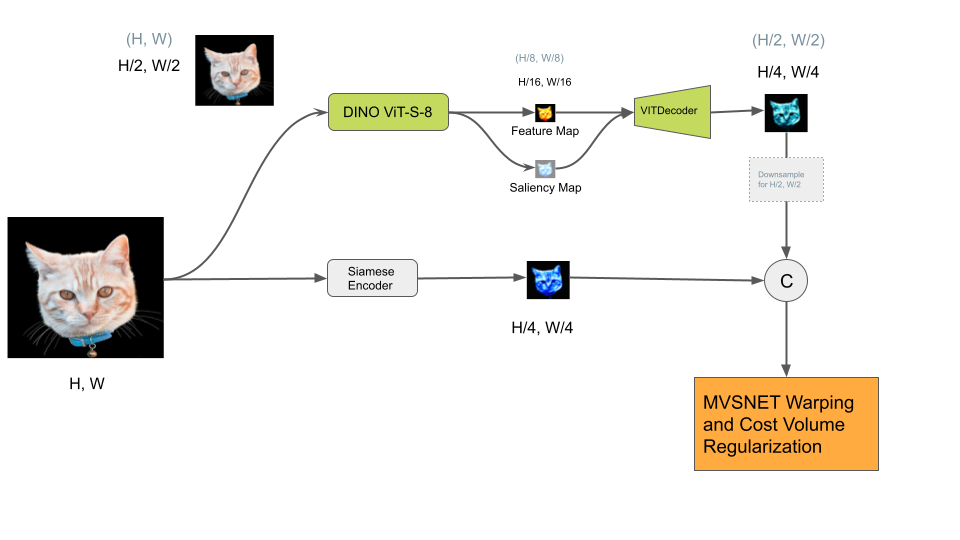
\includegraphics[width=1\textwidth]{images/vit.png}
      \caption[Using ViT features to augment learned features]{\textbf{Using ViT features to augment learned features.} Here, we see how features and saliency maps obtained from the pretrained DINO-ViT-S-8 backbone are used to augment the learned features from {\mvsn} siamese encoder. The final size of the features and saliency maps obtained from the ViT is \(\frac{H}{16}, \frac{W}{16}\). These features and saliency maps are then fused and upscaled to \(\frac{H}{4}, \frac{W}{4}\) by the VITDecoder module\cite{cao2022mvsformer}. For the setting where the ViT feature extractor is given the full-sized images as input (in Grey), we downsample the fused output of the ViTDecoder by a factor of \(\frac{1}{2}\) (shown by the dotted grey rectangle) before concatenating with the learned features from the Siamese encoder.}
\label{fig:vit}
\end{figure}
    
    
    
    \item \textbf{RobustMVD Base: Switching out the DispNet feature encoder in RobustMVD and replacing it with the {\mvsn} encoder.:} Consequently, based on the findings of previous experiments, it is prudent to investigate the impact of replacing the feature encoder in DispNet with the {\mvsn} feature encoder. Our goal was to evaluate whether the distinctive features extracted by {\mvsn}'s encoder would enhance or degrade the performance of DispNet. Initially, the {\mvsn} encoder was incompatible with the DispNet architecture. Therefore, we had to adapt the {\mvsn} encoder for effective integration. Our adaptation involved several significant changes. \par

    Firstly, we increased the initial number of feature channels from 8 to 64. This leads to an increase in the number of channels in the extracted features of the {\mvsn} encoder from 32 to 256. This decision, although initially based on the need to make the {\mvsn} encoder compatible with the rest of the DispNet architecture, also has the added benefit of potentially extracting more complex features from the input images and maintaining the deeper architecture of the {\mvsn} encoder, acknowledging the trade-off of increased computational complexity.\par
    
    Secondly, we adjusted the stride of the first convolutional layer from 1 to 2. This allowed the convolutional filters to skip every other pixel, reducing the output size and computational cost while constructing the correlations and the cost volume. We perform this change to maintain the spatial dimensions of the skip connections from the {\mvsn} encoder to the DispNet decoder. Note that this operation might lead to the loss of some fine-grained detail due to the reduction in input size. \par

    In the original {\mvsn} encoder, every convolution layer uses batch normalization. We changed this in our modified encoder. Specifically, the last convolution layer of each block ($conv1b$, $conv2c$, and $conv3c$ in \hyperref[tab:arch-mvsn]{Table2.1}) was implemented without batch normalization. $conv1b$ and $conv2c$ are fed as skip connections to the decoder part of the cost volume regularization network (refer to \hyperref[tab:arch-mvsn]{Table2.5} for details of the skip connections). Although batch normalization generally improves the speed, performance, and stability of a neural network, we found that, in our case, it led to training divergence. This phenomenon might have been due to the model's increased sensitivity to changes in the distribution of each layer's input, leading to amplified noise or exploding gradients. Therefore, to stabilize our training, we removed it from the last layers. It should be noted that the GC-Net\cite{kendall2017end} architecture also removes BatchNorm and ReLU for the layers whose outputs are used as skip connections to the cost volume regularization network. \par
    
    Another significant modification was removing the $conv3r$ layer from the {\mvsn} encoder. The $conv3r$ layer is initially used to increase the depth of the encoder without changing the spatial dimensions of the output through the use of a 1x1 kernel, potentially facilitating the learning of more complex representations.  It should be noted from \hyperref[tab:arch-rmvd]{Table 3.}{2} that the DispNet architecture has an additional component, the \textit{Context Encoder}, which comes after the feature encoder. It contains a layer, $conv3a_0$, that performs a 1x1 convolution to reduce the depth of the feature map from 256 to 32 while maintaining the spatial dimensions in a similar fashion to the function of the $conv3r$ layer in the original {\mvsn} encoder (refer to \hyperref[tab:arch-mvsn]{Table 2.}{1}). The encoded context obtained from this layer is concatenated to the output of the cost volume fusion layer further down into the network before passing the concatenated tensor to the cost volume regularization layer. By removing the $conv3r$ layer from the original {\mvsn} encoder, we bridged the gap between the two different encoder architectures. We initially tried incorporating the $conv3r$ and the \textit{Context Encoder} in the network. However, including both components led to a divergence in training. Therefore, we removed the final $conv3r$ layer from the {\mvsn} encoder and directly used the output of $conv3c$. \par
    
    During the evaluation, the model trained on {\bms} showed a slight degradation in performance, as seen in \hyperref[tab:feat-enc]{Table 6b.2}. This is counter-intuitive to our expectation of a performance increase given the increase in depth offered by the {\mvsn} encoder and our modification to increase the feature channels from 32 to 256.\par
    We also trained this configuration with {\brs}, and there was a slight performance increase compared to its respective baseline of {\rmvd} trained with {\brs} as seen in \hyperref[tab:feat-enc]{Table 6b.1}. This highlights the sensitivity of the models to the variants of the datasets and batch sizes for training and its consequent effects on the evaluation. We will explore this further in the \hyperref[sec:exp-dataset-prop]{Section 5.3} on the properties of the data and datasets. 


\end{enumerate}

\subsection{Choice of Correlation Layer}\label{subsec:cvc}
In this section, we first take a look at the different types of correlation layers employed in our baseline models as well as in our experiments. We then discuss the results of the experiments in detail.
%\begin{table*}[t!]
\begin{table}[ht!]
\def\arraystretch{1.5}
\begin{adjustbox}{width=1\textwidth}
%\resizebox{\columnwidth}{!}{ % scale to columnwidth
%\resizebox*{\textwidth}{!}{
\setlength{\tabcolsep}{1mm}
\begin{tabular}{|l
|c c
|c c
|c c
|c c
|c c
||c |c |c |c |c
|}

\hline
    \textbf{Correlation Layer w/o}
    & \multicolumn{2}{c|}{\textbf{\kittishort{}}}
    & \multicolumn{2}{c|}{\textbf{\dtushort{}{}}}
    & \multicolumn{2}{c|}{\textbf{\scannetshort{}}}
    & \multicolumn{2}{c|}{\textbf{\tanksandtemplesshort{}}}
    & \multicolumn{2}{c|}{\textbf{\ethdshort{}}}
    & \multicolumn{5}{c|}{\textbf{Average}}
    \\
\hline
    \textbf{Normalized Features}
    & $\absrel\downarrow$ & $\threshI\uparrow$
    & $\absrel\downarrow$ & $\threshI\uparrow$
    & $\absrel\downarrow$ & $\threshI\uparrow$
    & $\absrel\downarrow$ & $\threshI\uparrow$
    & $\absrel\downarrow$ & $\threshI\uparrow$
    & $\absrel\downarrow$ & $\threshI\uparrow$ & AUSE$ \downarrow$ & time $\downarrow$ & memory $\downarrow$
    \\

    &&&&&&&&&&&&&&(mSec)&(MB)\\
    \hline
    \hline

    \textbf{a) {\mvsn} Base}
	& 
	& 
	& 
	& 
	& 
	& 
	& 
	& 
	& 
	& 
	& 
	& 
 	& 
	& 
	& 
    \\
\hline
\rowcolor{bgcolor}
    \textbf{a1) Default Training and}
	& 
	& 
	& 
	& 
	& 
	& 
	& 
	& 
	& 
	& 
	& 
	& 
        & 
	& 
	& 
        \\
\rowcolor{bgcolor}
    \textbf{    Evaluation Input sizes}
	& 
	& 
	& 
	& 
	& 
	& 
	& 
	& 
	& 
	& 
	& 
	& 
        & 
	& 
	& 
        \\
\hdashline
\rowcolor{bgcolor}
	MVSNet Base $(V=2, D=128)$
	& 11.44
	& 40.50
	& 2.95
	& 81.26
	& 9.80
	& 32.31
	& 9.31
	& 80.24
	& 31.45
	& \bestresult{38.51}
	& 12.99
	& \bestresult{55.56}
        & \bestresult{0.26}
        & 65.2
        & 5302
	
	\\ 

\hline
	Groupwise ($G=4$) with
 	& 
	& 
	& 
	& 
	& 
	& 
	& 
	& 
	& 
	& 
	& 
	& 
 	& 
	& 
	& 
	\\ 
        Learned Fusion 
	& 9.90
	& 40.89
	& 3.17
	& \bestresult{81.40}
	& 8.86
	& 33.22
	& \bestresult{6.59}
	& \bestresult{80.80}
	& 21.43
	& 38.06
	& 9.99
	& 54.87
        & 0.27
        & \bestresult{34.23}
        & \bestresult{3153}
	\\ 
\hline
	Groupwise ($G=4$) + WarpOnly
 	& 
	& 
	& 
	& 
	& 
	& 
	& 
	& 
	& 
	& 
	& 
	& 
 	& 
	& 
	& 
	\\ 
        with Learned Fusion 
	& \bestresult{8.17}
	& \bestresult{43.59}
	& 4.01
	& 78.52
	& \bestresult{8.58}
	& \bestresult{34.98}
	& 6.71
	& 80.18
	& \bestresult{19.21}
	& 38.09
	& \bestresult{9.34}
	& 55.07
        & 0.28 
        & 84.28
        & 8527
	\\ 
	
    \hline
    \hline

    \textbf{b) {\rmvd} Base}
	& 
	& 
	& 
	& 
	& 
	& 
	& 
	& 
	& 
	& 
	& 
	& 
 	& 
	& 
	& 
    \\

\hline
\rowcolor{bgcolor}
        \textbf{b1) Train on {\bms}} 
        & 
	& 
	& 
	& 
	& 
	& 
	& 
	& 
	& 
	& 
	& 
	& 
        & 
	& 
	& 
        \\
\rowcolor{bgcolor}
    \textbf{and reduced Evaluation Input sizes}
	& 
	& 
	& 
	& 
	& 
	& 
	& 
	& 
	& 
	& 
	& 
	& 
        & 
	& 
	& 
        \\
\hdashline
\rowcolor{bgcolor}
{\rmvd} Base $(V=2 , B=1)$ \(\star\)
	& \bestresult{8.21}
	& \bestresult{35.51}
	& \bestresult{4.24}
	& \bestresult{71.04}
	& \bestresult{9.06}
	& \bestresult{31.07}
	& 11.34
	& \bestresult{60.78}
	& \bestresult{11.13}
	& \bestresult{36.58}
	& \bestresult{8.80}
	& \bestresult{47.00}
        & 0.28
        & \bestresult{25.23}
        & \bestresult{1136}
	\\ 
    \hline
        Groupwise $(G=4)$ with 
        & 
	& 
	& 
	& 
	& 
	& 
	& 
	& 
	& 
	& 
	& 
	& 
 	& 
	& 
	& 
    \\
	Learned Fusion (600k iterations) 
	& 10.21
	& 30.50
	& 4.92
	& 69.04
	& 38.84
	& 30.21
	& 9.59
	& 55.03
	& 15.29
	& 31.05
	& 15.77
	& 43.16
        & \bestresult{0.26}
        & 64.1
        & 7374
	\\ 
        and 2D cost regularization \(\star\)
	& 
	& 
	& 
	& 
	& 
	& 
	& 
	& 
	& 
	& 
	& 
	& 
 	& 
	& 
	& 
	\\ 
\hline
        Groupwise $(G=4)$ with 
        & 
	& 
	& 
	& 
	& 
	& 
	& 
	& 
	& 
	& 
	& 
	& 
 	& 
	& 
	& 
    \\
	Learned Fusion (1000k iterations)
        & 9.49
	& 30.09
	& 4.38
	& 71.04
	& 39.83
	& 30.14
	& \bestresult{7.37}
	& 56.49
	& 13.89
	& 32.43
	& 14.99
	& 44.04
        & 0.27
        & 61.38
        & 7370
    \\ 
        and 2D cost regularization \(\star\)
	& 
	& 
	& 
	& 
	& 
	& 
	& 
	& 
	& 
	& 
	& 
	& 
 	& 
	& 
	& 
	\\ 
\hline
        Groupwise $(G=4)$ + Full Corr 
	& 
	& 
	& 
	& 
	& 
	& 
	& 
	& 
	& 
	& 
	& 
	& 
 	& 
	& 
	& 
	\\ 
        with Learned fusion and
	& 32.21
	& 12.91
	& 5868.07
	& 0
	& 2061.13
	& 0.63
	& 96.27
	& 14.69
	& 795.89
	& 5.01
	& 1770.71
	& 6.65
        & 0.35
        & 127.32
        & 7504
	\\ 
         3D cost regularization \(\star\)
        & 
	& 
	& 
	& 
	& 
	& 
	& 
	& 
	& 
	& 
	& 
	& 
 	& 
	& 
	& 
	\\ 

	
\hline




	

\end{tabular}
\end{adjustbox}
\caption[Changing the correlation layer]{\textbf{Changing the correlation layer}.
\textbf{a)} All {\mvsn} and {\rmvd} derivatives are trained on {\bms}. In \textbf{a.1}, we can see that both implementations with {\gwc} (GWC) and the GWC combined with differential homography outperform the baseline. The model using only GWC as a correlation layer has a significantly lesser inference time and memory requirement. In \textbf{b.1}, all our implemented models for {\rmvd} using GWC perform very poorly compared to the baseline. Due to the high memory requirements of GWC for {\rmvd} due to 256 channels in the feature maps, we use the smaller evaluation inputs. This is indicated by a \(\star\). The baselines are shaded in grey.
\label{tab:corr-layer}
}
\end{table}

%\end{table*}

\begin{enumerate}
    \item \textbf{Plane sweep based Warping}\cite{Yao2018}: As the name suggests, this is not really a correlation operation. This operation was used first in {\mvsn} and later in some of its extensions \cite{Gu2020, yang2019hierarchical, Yao2019} to warp the source features to the reference image frustum at different depth levels and build a cost volume. Consequently, these methods also use a variance-based cost volume fusion methodology, which looks at the variance between the warped source features and the reference features. We saw the working of this in \hyperref[sec:multiviewster]{Section 4} of the Background chapter. 
    \item \textbf{Full Correlation} \cite{Mayer2016}: The Full Correlation, was introduced for the first time in the DispNet paper. The Full correlation is computed as per the following equation.
    \begin{equation}
        c(\mathcal{F}_{ref}, \mathcal{F}_{source}) = \langle \mathcal{F}_{ref} , \mathcal{F}_{source}^T \rangle
    \end{equation} where $\langle:,:\rangle$ denotes matrix multiplication.
    This operation contains  \(C \times W^2\times H^2\) multiplications, is computationally intensive, and is performed for each pair of source and reference images. Here \(C\) is the number of channels in the feature maps of the reference and source images. We can see that this operation decimates the feature dimension of the two feature maps. The correlation map has dimensions ($B \times (W\times H) \times (W\times H)$). It contains matching similarity costs between the key view pixels and points on their respective epipolar lines in the source view for a set of sampled inverse depth values. The individual correlation maps are then fused together with a learned weights fusion or simply averaging them together. {\rmvd} uses this correlation method to obtain a 2D cost map. 
    \item \textbf{{\gwc}} \cite{guo2019group}: {\gwc} (GWC) was first used by Guo {\etal} to calculate the similarity between the left and right images in stereo matching by disparity estimation. This thesis extends it to the depth estimation with the MVS scenario. After the initial warping step, we the source features warped at each depth level with a projection of the reference features along the depth of the frustum. Unlike traditional correlation, which calculates the similarity between pixels along all feature channels, {\gwc} considers a group of channels simultaneously. The {\gwc} volume is computed as follows: 
    \begin{enumerate}
        \item Given the warped and projected source and projected reference features of dimensions \((B, C, D, H, W)\), we reshape them into tensors of shape \((B, G, \frac{C}{G}, D, H, W)\). Here, \(G\) is the number of groups. 
        \item We then take an element-wise inner product between the reshaped tensors and sum over the \(\frac{C}{G}\) or the group-channels dimension.
        \item The cost volume obtained \(V_{gwc}\) has a shape \((B, G, D, H, W)\) and is given as: 

            \[V_{gwc} =\Sigma_{group-channels} (A \odot B)\]

        where $A$ is the reference feature and \(B\) is the warped source feature projected along the depth of the frustum. And \(\odot\) represents the element-wise inner product. The summation operation is performed along the \(\frac{C}{G}\) dimension after taking the product. We used learned fusion to fuse the individual cost volumes. 
    \end{enumerate}
\end{enumerate}
It should be noted that since the correlation layer and the subsequent fusion operation are the most defining parts of an {\mvs} pipeline, we do not switch the full correlation and the differential homography between {\rmvd} and {\mvsn}. Instead, we perform two different types of experiments. In the first type, we replace the existing correlation layer with {\gwc} and use learned fusion to fuse the individual pairwise cost volumes while retaining the remaining architecture as it is. In the second type, we concatenate the output of the original correlation layer of the model with the output of the {\gwc} and use learned fusion to fuse the concatenated volumes. The fused volume is then given as input to either a 3D or 2D cost volume regularization network. \par

For our experiments, we set the value of \(G\) to 4. From \hyperref[tab:corr-layer]{Table 7a.}{1}, we can see that {\gwc} outperforms our {\mvsn} baseline by a significant margin. We also implemented a {\mvsn} multi-correlation model that computes both plane sweep warping volume and {\gwc} volume for each reference and source pair. We then concatenate both volumes and fuse the individual concatenated volumes using learned fusion by computing the weights for each concatenated volume. This model outperforms both the baseline and the model with only {\gwc}. 

For {\rmvd}, it should be noted that the models are trained on the {\bms}, which contains two best views and a batch size of 1. In \hyperref[tab:corr-layer]{Table 7b.}{1}, we observe a significant reduction in performance compared to the respective baseline. We include an additional layer to the architecture called the \textit{CostVolume3DContextEncoder}. This contains three 3D convolutional layers, each with a kernel size of one, to reduce the number of channels in \(V_{gwc}\) from \(G\) to 1. We then squeezed the channel dimension and used the 2D DispNet cost volume regularization network to regress the depth and the uncertainty maps from this reduced cost volume. We conjectured that the model needed more time to learn the additional weights, so we trained it for 1000000 iterations instead of the usual 600000. We observed a slight improvement in performance for the model that was trained for a longer period; however, it was not enough to justify the continuation of training. \par

The third experiment for {\rmvd} consists of the concatenation of the output of the {\gwc} operation and the Full correlation operation. Since the full correlation output does not have an explicit channel dimension, we unsqueeze the tensor at the first dimension and concatenate it to the output of the GWC layer. We further concatenate the output of the context encoder unit of the {\rmvd} model (refer to \hyperref[tab:arch-rmvd]{Table 3.}{2}) to this by expanding it along the depth dimension. This concatenated tensor is then passed on to the 3D cost volume regularization network. In \hyperref[tab:corr-layer]{Table 7b.}{1} in the third entry, we can see that this model performs very poorly compared to the baseline and the other implemented models. 
\subsection{Choice of Cost Volume Fusion Method}\label{subsec:cvf}
%\begin{table*}[t!]
\begin{table}[ht!]
\def\arraystretch{1.5}
\begin{adjustbox}{width=1\textwidth}
%\resizebox{\columnwidth}{!}{ % scale to columnwidth
%\resizebox*{\textwidth}{!}{
\setlength{\tabcolsep}{1mm}
\begin{tabular}{|l
|c c
|c c
|c c
|c c
|c c
||c |c |c |c |c
|}

\hline

    \textbf{Fusion Method}
    & \multicolumn{2}{c|}{\textbf{\kittishort{}}}
    & \multicolumn{2}{c|}{\textbf{\dtushort{}{}}}
    & \multicolumn{2}{c|}{\textbf{\scannetshort{}}}
    & \multicolumn{2}{c|}{\textbf{\tanksandtemplesshort{}}}
    & \multicolumn{2}{c|}{\textbf{\ethdshort{}}}
    & \multicolumn{5}{c|}{\textbf{Average}}
    \\
\hline
    & $\absrel\downarrow$ & $\threshI\uparrow$
    & $\absrel\downarrow$ & $\threshI\uparrow$
    & $\absrel\downarrow$ & $\threshI\uparrow$
    & $\absrel\downarrow$ & $\threshI\uparrow$
    & $\absrel\downarrow$ & $\threshI\uparrow$
    & $\absrel\downarrow$ & $\threshI\uparrow$ & AUSE$ \downarrow$ & time $\downarrow$ & memory $\downarrow$
    \\

    &&&&&&&&&&&&&&(mSec)&(MB)\\
    \hline
    \hline

    \textbf{a) {\mvsn} Base}
	& 
	& 
	& 
	& 
	& 
	& 
	& 
	& 
	& 
	& 
	& 
	& 
 	& 
	& 
	& 
    \\
    \hline
    \rowcolor{bgcolor}
    \textbf{a1) Default Training and}
	& 
	& 
	& 
	& 
	& 
	& 
	& 
	& 
	& 
	& 
	& 
	& 
        & 
	& 
	& 
        \\
\rowcolor{bgcolor}
    \textbf{    Evaluation Input sizes}
	& 
	& 
	& 
	& 
	& 
	& 
	& 
	& 
	& 
	& 
	& 
	& 
        & 
	& 
	& 
        \\
\hdashline
\rowcolor{bgcolor}
	MVSNet Base $(V=2, D=128)$
	& \bestresult{11.44}
	& \bestresult{40.50}
	& \bestresult{2.95}
	& \bestresult{81.26}
	& \bestresult{9.80}
	& \bestresult{32.31}
	& \bestresult{9.31}
	& \bestresult{80.24}
	& \bestresult{31.45}
	& \bestresult{38.51}
	& \bestresult{12.99}
	& \bestresult{55.56}
        & \bestresult{0.26}
        & 65.2
        & 5302
	
	\\ 

\hline
	{\mvsn} with Learned Fusion
	& 27.53
	& 10.48
	& 9.71
	& 49.54
	& 15.52
	& 17.25
	& 12.73
	& 50.88
	& 38.42
	& 16.50
	& 20.78
	& 28.93
        & 0.39
        & 37.21
        & 5732
	\\ 
 \hline
	{\mvsn} with Average Fusion
	& 37.42
	& 10.44
	& 9.29
	& 48.40
	& 16.91
	& 18.91
	& 14.28
	& 47.44
	& 40.21
	& 14.36
	& 22.06
	& 27.87
        & 0.37
        & \bestresult{35.82}
        & \bestresult{4322}
	\\

\hline
\hline
        \textbf{b){\rmvd} Base}
	& 
	& 
	& 
	& 
	& 
	& 
	& 
	& 
	& 
	& 
	& 
	& 
 	& 
	& 
	& 
	\\
 \hline
 \rowcolor{bgcolor}
        \textbf{b1) Train on {\bms}} 
        & 
	& 
	& 
	& 
	& 
	& 
	& 
	& 
	& 
	& 
	& 
	& 
        & 
	& 
	& 
        \\
\rowcolor{bgcolor}
    \textbf{and default Evaluation Input sizes}
	& 
	& 
	& 
	& 
	& 
	& 
	& 
	& 
	& 
	& 
	& 
	& 
        & 
	& 
	& 
        \\
\hdashline
\rowcolor{bgcolor}
{\rmvd} Base $(V=2 , B=1)$ 
	& \bestresult{8.22}
	& \bestresult{35.51}
	& 4.74
	& 68.00
	& 9.06
	& 31.07
	& 12.58
	& 62.87
	& \bestresult{11.58}
	& 36.60
	& 9.24
	& 46.81
        & 0.28
        & \bestresult{30.24}
        & 2125
	\\ 
 \hline
        {\rmvd} with Average Fusion \((V=2)\)
	& 8.99
	& 34.82
	& \bestresult{4.06}
	& \bestresult{73.66}
	& \bestresult{8.83}
	& \bestresult{31.68}
	& \bestresult{9.91}
	& \bestresult{65.65}
	& 13.34
	& \bestresult{39.16}
	& \bestresult{9.02}
	& \bestresult{48.99}
        & \bestresult{0.26}
        & 45.53
        & \bestresult{1783}
	\\ 
	


	
\hline
\end{tabular}
\end{adjustbox}
\caption[Changing the cost volume fusion layer]{\textbf{Changing the cost volume fusion layer}.
\textbf{a)} For experiments with the fusion layer, both {\mvsn} derivatives and {\rmvd} derivatives are trained on {\bms}. A variance-based fusion only makes sense if there is only warping and no correlation computation between the reference and source features, as in {\mvsn}. In \textbf{a.1}, we can see that both learned fusion and average fusion don't work well with {\mvsn} for this reason. Consequently, we omit the combination {\rmvd} with Variance Fusion because {\rmvd} computes the full correlation between the reference and the source features. In \textbf{b.1}, we can see that average fusion gives slightly better results for average fusion compared to learned fusion for the given number of views. It should be noted that this might not necessarily be the case if the same experiment is repeated with a larger number of source views. 
\label{tab:cvf}
}
\end{table}

%\end{table*}

\begin{enumerate}
    \item \textbf{Variance Fusion} \cite{Yao2018}: This is used in the baseline {\mvsn} model. Variance-based fusion of individual cost volumes operates on the principle that all views contribute equally to the final fused cost volume. A cost metric based on variance is only applicable in models that utilize a differential homography warping approach, as correlation computation between reference and source features is not explicitly performed during the homography warping process.\hyperref[tab:arch-mvsn]{Table 2.3} gives the equation to obtain the fused cost volume from the individual cost volumes. We only use variance-based fusion for some {\mvsn} derivatives that only warp the source features to the reference features, as the cost volumes generated by any model that computes correlations cannot be fused with a variance metric. Hence, we cannot fuse the full correlations of {\rmvd} with variance fusion.  
    \item \textbf{Learned Fusion}\cite{schroeppel2022benchmark, Hartmann2017}: In learned fusion, we pass the individual cost volumes through a small 2D or 3D CNN network to learn the respective weights for each volume. First, we utilize the per-pixel (for 2D cost maps) or voxel weights (for 3D cost volumes) that we acquired. We applied these weights to each individual volume and then calculated a weighted average to produce the final fused cost volume. Unlike the variance operation, learned fusion can be used for derivatives of {\mvsn} that employ a different correlation layer other than the differential warping and {\rmvd}. Therefore, as part of our ablation study, we implemented {\mvsn} with learned fusion. In \hyperref[tab:cvf]{Table 8a.1}, we can see that the learned fusion for {\mvsn} performed much worse than the variance-based fusion baseline. This is because variance-based fusion implicitly computes the similarity between reference and individual warped source volumes instead of explicitly computing the correlation between the two. Hence, learned fusion does not work well in such a scenario, with no actual matching costs in the cost volume. We used learned fusion extensively in our models, where the correlation is computed explicitly in the correlation layer, such as the {\mvsn} models using {\gwc} as a correlation layer in the previous section. 
    \item \textbf{Average Fusion}\cite{im2019dpsnet}: Average fusion, like learned fusion, can be used for both {\mvsn} and {\rmvd} models. In \hyperref[tab:cvf]{Table 8a.1}, we can see the performance is slightly worse than the learned fusion for {\mvsn} and significantly worse than the baseline based on variance fusion. In \hyperref[tab:cvf]{Table 8b.1} {\rmvd} with average fusion performs slightly better than our baseline model, which uses a learned fusion strategy. Schröppel \etal demonstrates this by training {\rmvd} with average fusion using four views instead of two. This model exhibits a slightly lower performance than the baseline {\rmvd} model trained with learned fusion. \cite{schroeppel2022benchmark}
\end{enumerate}
\subsection{Choice of Cost Volume Regularization Network Component}\label{subsec:cvr}
%\begin{table*}[t!]
\begin{table}[ht!]
\footnotesize
\centering
\def\arraystretch{1.5}
%\resizebox{\columnwidth}{!}{ % scale to columnwidth
%\resizebox*{\textwidth}{!}{
\begin{adjustbox}{width=1\textwidth}
\setlength{\tabcolsep}{1mm}
\begin{tabular}{|l
|c c
|c c
|c c
|c c
|c c
||c |c |c |c |c
|}

\hline

    \textbf{Cost Vol Regularization}
    & \multicolumn{2}{c|}{\textbf{\kittishort{}}}
    & \multicolumn{2}{c|}{\textbf{\dtushort{}{}}}
    & \multicolumn{2}{c|}{\textbf{\scannetshort{}}}
    & \multicolumn{2}{c|}{\textbf{\tanksandtemplesshort{}}}
    & \multicolumn{2}{c|}{\textbf{\ethdshort{}}}
    & \multicolumn{5}{c|}{\textbf{Average}}
    \\
\hline
    & $\absrel\downarrow$ & $\threshI\uparrow$
    & $\absrel\downarrow$ & $\threshI\uparrow$
    & $\absrel\downarrow$ & $\threshI\uparrow$
    & $\absrel\downarrow$ & $\threshI\uparrow$
    & $\absrel\downarrow$ & $\threshI\uparrow$
    & $\absrel\downarrow$ & $\threshI\uparrow$ & AUSE$ \downarrow$ & time $\downarrow$ & memory $\downarrow$
    \\
    &&&&&&&&&&&&&&(mSec)&(MB)\\
    \hline
    \hline
    \textbf{a) {\mvsn} Base}
	& 
	& 
	& 
	& 
	& 
	& 
	& 
	& 
	& 
	& 
	& 
	& 
 	& 
	& 
	& 
    \\
\hline
    \rowcolor{bgcolor}
    \textbf{a1) Default Training and}
	& 
	& 
	& 
	& 
	& 
	& 
	& 
	& 
	& 
	& 
	& 
	& 
        & 
	& 
	& 
        \\
\rowcolor{bgcolor}
    \textbf{    Evaluation Input sizes}
	& 
	& 
	& 
	& 
	& 
	& 
	& 
	& 
	& 
	& 
	& 
	& 
        & 
	& 
	& 
        \\
\hdashline
\rowcolor{bgcolor}
	MVSNet Base $(V=2, D=128)$
	& 11.44
	& 40.50
	& 2.95
	& 81.26
	& 9.80
	& 32.31
	& 9.31
	& 80.24
	& 31.45
	& 38.51
	& 12.99
	& 55.56
        & 0.26
        & 65.2
        & \bestresult{5302}
	
	\\ 

\hline
	DispNet 2D Decoder 
	& \bestresult{7.79}
	& \bestresult{48.92}
	& 2.83
	& 83.22
	& \bestresult{8.20}
	& \bestresult{36.84}
	& \bestresult{5.75}
	& \bestresult{83.76}
	& \bestresult{19.26}
	& \bestresult{40.63}
	& \bestresult{8.77}
	& \bestresult{58.67}
        & 0.29
        & 627.45
        & 5491
	\\ 
\hline
     3D UNet Stacked Hourglass
	& 10.63
	& 39.58
	& \bestresult{2.64}
	& \bestresult{85.33}
	& 9.96
	& 32.90
	& 6.13
	& 81.82
	& 25.73
	& 38.31
	& 11.02
	& 55.59
        & \bestresult{0.25}
        & \bestresult{45.54}
        & 5373
    \\
	



\hline
\end{tabular}
\end{adjustbox}
\caption[Changing the cost volume regularization layer]{\textbf{Changing the cost volume regularization layer}.
\textbf{a)} All {\mvsn} derivatives are trained on {\bms}. It is evident that both of our models outperform the baseline. Particularly, the implementation of {\mvsn} using a 2D DispNet decoder shows significant improvement over the baseline. However, we can see that it takes significantly longer to make inferences compared to the baseline. In the second entry, we see that applying the Stacked Hourglass regularization yields better results than the baseline without causing a significant increase in inference time and memory requirements.
\label{tab:cvr}
}
\end{table}

%\end{table*}

\begin{enumerate}
    \item \textbf{Switching out the MVSNet fused cost-volume decoder with the DispNet fused cost-volume decoder.:} In the original MVSNet, the cost volume is a 3D volume with dimensions (Batch size, Channels, Depth levels, Height, Width). Here, each pixel across all depth planes is associated with a probability of that pixel at that depth being part of the object surface in the scene. It is a structured cost volume that is then passed to a 3D CNN Encoder Decoder cost volume regularization component. Now, since we wanted to switch to the DispNet cost volume decoder, which is a 2D decoder, we deal with this problem by slicing the fused cost volume along the depth dimension in a similar fashion to \cite{Yao2019}. \par
    
    The simplest way to integrate the 3D fused cost volume into a 2D decoder is to slice it at each depth level and pass each layer individually to the 2D decoder. The output of each layer could then be interpreted as a probability map for that depth. The depth map can then be obtained by choosing the depth with the maximum probability for each pixel. However, this increases the time complexity, as the 2D decoder needs to process the image once for each depth layer. \par
    The skip connections from the fused cost volume encoder are also three-dimensional. However, since they are intermediary representations, they have a larger number of depth levels compared to the final output of the cost volume encoder. To reconcile this difference, we use trilinear interpolation to match the slices from intermediate volumes with fewer depth dimensions, including the final output, to those of the output with the largest depth dimension, which in our case is $3DConv0$. For instance, given that we have volumes of sizes (1, 64, 32, 4, 5) and (1, 32, 64, 8, 10), we interpolate along the depth dimension of the first volume to match the depth dimension of the second volume, which gives the new volume of shape (1, 64, 64, 4, 5). \par
    To preserve the spatial correlation between the slices, we maintain the order of the slices along the depth dimension, as it represents the spatial relationship between different depths. In this manner, we use the 3D skip connections in the 2D decoder by transforming the 3D volumes into a series of individual 2D depth planes, which we then feed into the 2D decoder at the appropriate layers. This process is visualized in \hyperref[fig:2ddec-3dcv]{Figure 6}.\par
    \begin{figure}[ht]
    \centering
     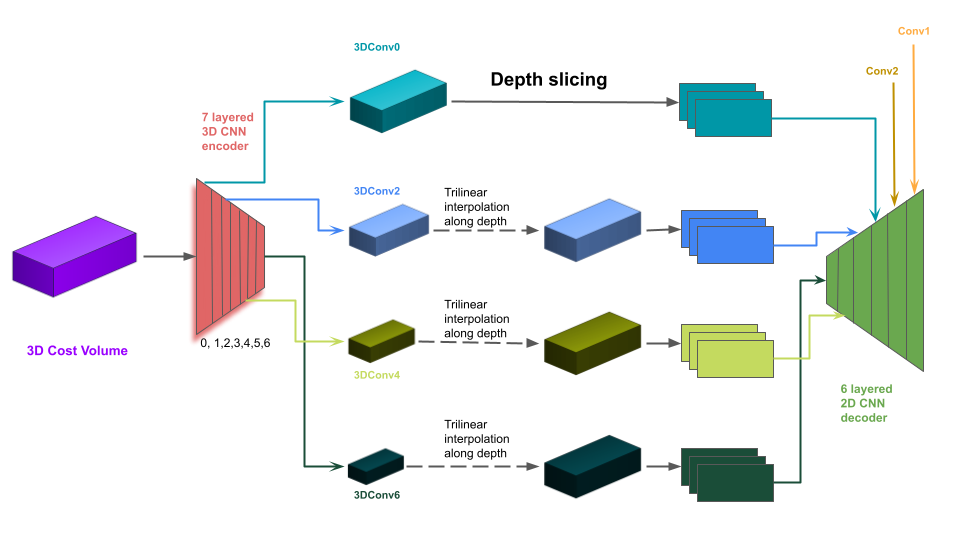
\includegraphics[width=1\textwidth]{images/2ddec-3dcv.png}
      \caption[Using a 2D Decoder for 3D Cost Volume Regularization]{\textbf{Using a 2D Decoder for 3D Cost Volume Regularization.} This figure shows the method of \textit{depth slicing} used to regularize a 3D cost volume using a 3D-2D hybrid Encoder-Decoder. The final and intermediate skip connection outputs of the 3D encoder are interpolated along the depth dimension to match the number of depth levels in each of them. Then, each \textit{depth slice} of the final encoder output, along with its corresponding depth slices from the intermediate representations, are sent individually to the 2D decoder for processing. The decoder outputs from each tuple of \textit{depth slices} are then stacked along the depth dimension, and the depth map is regressed from this cost volume. This final step is not shown in the figure.}
    \label{fig:2ddec-3dcv}
    \end{figure}
    This method takes longer to train than a normal 3D convolution decoder, as the decoder is called for each tuple of depth slices. These tuples look like ($3Dconv0[:,:,i,:,:]$, $3Dconv2[:,:,i,:,:]$, $3Dconv4[:,:,i,:,:]$, $3Dconv6[:,:,i,:,:]$). The maximum value of $i$ depends on the number of depth sampling points chosen at the beginning of the training, which in our case is $D=128$. In \hyperref[tab:cvr]{Table 9a.1}, we can see that this model gives much better results compared to the baseline of training {\mvsn} on {\bms} with $128$ depth samples. It also performs better than training {\mvsn} with $256$ depth values. The drawback of this model is that it takes a long time to train because each depth slice is processed by the cost volume decoder individually. The output of each iteration is aggregated into a new regularized cost volume along the depth dimension. The final depth map is regressed from this cost volume.\par 

    \item \textbf{{\mvsn} with Stacked Hourglass Cost Volume Regularization Network}: In this experiment, we implemented a stacked hourglass network, which is used for regularizing the raw fused cost volume. The architecture for this network is given in detail in \hyperref[tab:arch-stacked]{Table 16}{}. Each \textit{hourglass} in the architecture is an encoder-decoder network with skip connections going from the encoder to the decoder. Our architecture incorporates three distinct hourglass modules. After every level, a depth map is generated from the probability volume. To calculate the loss, we use a weighted summation of the smooth L1 loss between the depth maps and ground truth at each output level of the stacked hourglass. From \hyperref[tab:cvr]{Table 9a.1}, we can see that this model also performs better than the baseline without significantly increasing inference time and memory requirement. 

\end{enumerate}



\subsection{Usage of Coarse to Fine Architecture} \label{subsec:c2f}
For the experiments in this section, we re-engineered our baseline models in a coarse-to-fine design \cite{Gu2020}. We consider a three-stage design. The depth range in the first stage, \(R_1\), encompasses the entire depth range of the input scene. Subsequent stages use the previously predicted output to constrict this initial hypothesized range. Mathematically, this is given by \(R_{k+1} = R_k \times w_k\), where \(R_k\) is the hypothesis range at stage \(k\) and \(w_k < 1\) is the reduction factor. Similarly, the depth interval at the initial stage is symbolized as \(I_1\). This interval is relatively larger than that in conventional singular cost volume formulations used in our baselines, making the primary depth estimation coarser. For subsequent stages, we use narrower intervals to derive finer-grained outputs. This can be written as \(I_{k+1} = I_k \times p_k\), where \(I_k\) is the hypothesis plane interval during the \(k^{th}\) stage and \(p_k < 1\) is the decrement factor. For stage \(k\), the total number of hypothesis planes, \(D_k\), is computed as \(D_k = \frac{R_k}{I_k}\). We use a value of \(p_k =\frac{1}{2}\). We use [32, 16, 8] depth hypotheses from the coarsest to the finest level. The interval ratios are set to [4, 2, 1]. This is such that the product of the interval ratio and the number of depth hypotheses at the coarsest level $32\times4=128$, which is equal to the number of depth hypotheses that we use for a single stage {\mvsn} model\cite{Gu2020}. The cascade formulation reduces the overall count of hypothesis planes as we refine the initial depth range in subsequent stages. Similar to \hyperref[eq:homography]{Equation 11}, the homography warping function for the \(k + 1^{th}\) stage can be reformulated as:
\begin{equation}
H_i(d^m_k + \Delta^m_{k+1}) = K_i \cdot R_i \cdot (I - \frac{(t_1 - t_i) \cdot n^T_1}{d^m_k + \Delta^m_{k+1}}) \cdot R^T_1 \cdot K^{-1}_1 \cdot d^m_k
\end{equation}
Here, \(d^m_k\) stands for the predicted depth of pixel \(m\) during the \(k^{th}\) stage, while \(\Delta^m_{k+1}\) represents the \(m^{th}\) pixel's residual depth for the \(k + 1^{th}\) stage\cite{zhu2021deep}.

We used the same smooth \(l1\) loss here as we did for our baselines with a slight modification. The predicted depth maps of each stage \(k\) are weighted by a factor \(\lambda_k\), and the total loss is the sum of all weighted losses. \par

In this section, we examine the impact of changing the feature extractors on the performance of models for coarse-to-fine design. Generating multilevel features is the most crucial component, so we focus on this. We trained the models using two different feature extractors: FPN and UNet. Unlike the FPN in \hyperref[subsec:fe]{Section 5.2.1}, we use a stride of one in the first $conv1a$ layer. Thus, the feature maps at each level have twice the resolution of the feature maps from the other implementation of FPN. These resolutions are given in \hyperref[tab:arch-fpn]{Table 13} in red. Similarly, for the UNet, we use all the features starting from \(feat2\) at the coarsest level and \(feat0\) at the finest level. This is possible due to the reduced number of depth hypotheses used in a coarse-to-fine architecture. 
Our experiments yielded results that are outlined in \hyperref[tab:c2f]{Table 10}. We observed that the {\mvsn} coarse-to-fine model with FPN feature extractor outperformed the baseline and had a much lower memory requirement, albeit requiring slightly more time for training and inference. This might be attributed to the adaptive number of depth levels and the cascading design of depth refinement. However, the UNet feature extractor-based coarse-to-fine design performed poorly compared to the baseline. Therefore, we can conclude that the FPN feature extractor is more suitable for a coarse-to-fine scenario than the UNet.

%\begin{table*}[t!]
\begin{table}[ht!]
\footnotesize
\centering
\def\arraystretch{1.5}
\begin{adjustbox}{width=1\textwidth}
%\resizebox{\columnwidth}{!}{ % scale to columnwidth
%\resizebox*{\textwidth}{!}{
\setlength{\tabcolsep}{1mm}
\begin{tabular}{|l
|c c
|c c
|c c
|c c
|c c
||c |c |c |c |c
|}

\hline

    \textbf{Feature Extractor for}
    & \multicolumn{2}{c|}{\textbf{\kittishort{}}}
    & \multicolumn{2}{c|}{\textbf{\dtushort{}{}}}
    & \multicolumn{2}{c|}{\textbf{\scannetshort{}}}
    & \multicolumn{2}{c|}{\textbf{\tanksandtemplesshort{}}}
    & \multicolumn{2}{c|}{\textbf{\ethdshort{}}}
    & \multicolumn{5}{c|}{\textbf{Average}}
    \\
\hline
    \textbf{Coarse-to-Fine}
    & $\absrel\downarrow$ & $\threshI\uparrow$
    & $\absrel\downarrow$ & $\threshI\uparrow$
    & $\absrel\downarrow$ & $\threshI\uparrow$
    & $\absrel\downarrow$ & $\threshI\uparrow$
    & $\absrel\downarrow$ & $\threshI\uparrow$
    & $\absrel\downarrow$ & $\threshI\uparrow$ & AUSE$ \downarrow$ & time $\downarrow$ & memory $\downarrow$
    \\

    &&&&&&&&&&&&&&(mSec)&(MB)\\
    \hline
    \hline
    \textbf{a) {\mvsn} Base}
	& 
	& 
	& 
	& 
	& 
	& 
	& 
	& 
	& 
	& 
	& 
	& 
 	& 
	& 
	& 
    \\
\hline
    \rowcolor{bgcolor}
    \textbf{a1) Default Training and}
	& 
	& 
	& 
	& 
	& 
	& 
	& 
	& 
	& 
	& 
	& 
	& 
        & 
	& 
	& 
        \\
\rowcolor{bgcolor}
    \textbf{    Evaluation Input sizes}
	& 
	& 
	& 
	& 
	& 
	& 
	& 
	& 
	& 
	& 
	& 
	& 
        & 
	& 
	& 
        \\
\hdashline
\rowcolor{bgcolor}
	MVSNet Base $(V=2, D=128)$
	& \bestresult{11.44}
	& \bestresult{40.50}
	& \bestresult{2.95}
	& \bestresult{81.26}
	& 9.80
	& 32.31
	& 9.31
	& 80.24
	& 31.45
	& \bestresult{38.51}
	& 12.99
	& \bestresult{55.56}
        & \bestresult{0.26}
        & \bestresult{65.2}
        & 5302
	
	\\ 
 \hline
	Cascade {\mvsn} with FPN FE
	& 16.11
	& 26.53
	& 3.31
	& 79.77
	& \bestresult{9.66}
	& 33.42
	& \bestresult{5.83}
	& \bestresult{81.55}
	& \bestresult{19.78}
	& 37.34
	& \bestresult{10.94}
	& 51.72
        & 0.88
        & 168.31
        & 2101
	\\ 
 \hline
	Cascade {\mvsn} with UNet FE
	& 24.15
	& 23.94
	& 3.21
	& 79.90
	& 10.20
	& \bestresult{33.69}
	& 7.66
	& 80.14
	& 25.85
	& 36.54
	& 14.22
	& 50.84
        & 0.86
        & 154.31
        & \bestresult{2044}
	\\

	
\hline
\end{tabular}
\end{adjustbox}
\caption[Changing the feature extractor for Coarse-to-Fine model design]{\textbf{Changing the feature extractor for Coarse-to-Fine model design}.
\textbf{a)}All {\mvsn} derivatives are trained on {\bms}. From the results, it is evident that the {\mvsn} coarse-to-fine model with FPN feature extractor outperforms the baseline. On the other hand, the model that has the UNet feature extractor performs poorly. Both models have a higher degree of uncertainty than the baseline and take longer to make inferences. However, the memory requirements for these models are significantly lower.
\label{tab:c2f}
}
\end{table}

%\end{table*}



\section{Effects of Changing Training Dataset Properties}\label{sec:exp-dataset-prop}
In this section, we analyze how modifying the properties of the input data impacts the model's performance. We do not make any changes to the test input data. All other settings are kept constant, and only a single attribute is changed in each experiment. All {\mvsn} models are given the camera intrinsics, poses, and depth range as input. All {\rmvd} models are given only the camera intrinsics and the poses as inputs. We do this to maintain similarity with the respective baselines. All {\rmvd} models are trained with Scale Augmentation unless explicitly specified. 
%\begin{table*}[t!]
\begin{table}[ht!]
\footnotesize
\centering
\def\arraystretch{1.5}
\begin{adjustbox}{width=1\textwidth}
%\resizebox{\columnwidth}{!}{ % scale to columnwidth
%\resizebox*{\textwidth}{!}{
\setlength{\tabcolsep}{1mm}
\begin{tabular}{|l
|c c
|c c
|c c
|c c
|c c
||c |c |c |c |c
|}

\hline

    \textbf{Approach}
    & \multicolumn{2}{c|}{\textbf{\kittishort{}}}
    & \multicolumn{2}{c|}{\textbf{\dtushort{}{}}}
    & \multicolumn{2}{c|}{\textbf{\scannetshort{}}}
    & \multicolumn{2}{c|}{\textbf{\tanksandtemplesshort{}}}
    & \multicolumn{2}{c|}{\textbf{\ethdshort{}}}
    & \multicolumn{5}{c|}{\textbf{Average}}
    \\
\hline
    & $\absrel\downarrow$ & $\threshI\uparrow$
    & $\absrel\downarrow$ & $\threshI\uparrow$
    & $\absrel\downarrow$ & $\threshI\uparrow$
    & $\absrel\downarrow$ & $\threshI\uparrow$
    & $\absrel\downarrow$ & $\threshI\uparrow$
    & $\absrel\downarrow$ & $\threshI\uparrow$ & AUSE$ \downarrow$ & time $\downarrow$ & memory $\downarrow$
    \\

    &&&&&&&&&&&&&&(mSec)&(MB)\\
    \hline
    \hline

    \textbf{a) Change Dataset}
	& 
	& 
	& 
	& 
	& 
	& 
	& 
	& 
	& 
	& 
	& 
	& 
 	& 
	& 
	& 
    \\
\hline
\rowcolor{bgcolor}
    \textbf{a1)} {\mvsn} Baseline \((V=2, D=128)\)
	& \bestresult{11.44}
	& \bestresult{40.50}
	& 2.95
	& 81.26
	& \bestresult{9.80}
	& \bestresult{32.31}
	& 9.31
	& \bestresult{80.24}
	& 31.45
	& \bestresult{38.51}
	& \bestresult{12.99}
	& \bestresult{55.56}
        & 0.26
        & \bestresult{65.2}
        & \bestresult{5302}
    \\
\hline
	{\mvsn} trained on {\dtushort{}{}} 
        & 
	& 
	& 
	& 
	& 
	& 
	& 
	& 
	& 
	& 
	& 
	& 
 	& 
	& 
	& 
    \\

        ($D=128, V=2$)
	& 18.67
	& 38.80
	& \bestresult{2.32}
	& \bestresult{85.84}
	& 12.17
	& 26.55
	& \bestresult{8.28}
	& 75.35
	& \bestresult{26.44}
	& 31.98
	& 13.57
	& 51.70
        & -
        & 112.73
        & 8716
	\\ 
    \hline
    \rowcolor{bgcolor}
        \textbf{a2)} {\rmvd} Baseline with
        & 
	& 
	& 
	& 
	& 
	& 
	& 
	& 
	& 
	& 
	& 
	& 
 	& 
	& 
	& 
    \\
\rowcolor{bgcolor}
    {\bms} \((V=2)\)
 	& \bestresult{8.22}
	& \bestresult{35.51}
	& 4.74
	& \bestresult{68.00}
	& \bestresult{9.06}
	& \bestresult{31.07}
	& \bestresult{12.58}
	& \bestresult{62.87}
	& \bestresult{11.58}
	& \bestresult{36.60}
	& \bestresult{9.24}
	& \bestresult{46.81}
        & 0.28
        & 30.24
        & 2125
    \\
    \hline
        {\rmvd} trained on {\dtushort{}{}} 
	& 
	& 
	& 
	& 
	& 
	& 
	& 
	& 
	& 
	& 
	& 
	& 
 	& 
	& 
	& 
	\\ 

        ($D=256, V=2$)
	& 48.16
	& 4.07
	& \bestresult{3.82}
	& 62.39
	& 33.70
	& 5.98
	& 50.80
	& 10.71
	& 51.14
	& 5.35
	& 37.53
        & 17.70
        & -
        & \bestresult{25.07}
        & \bestresult{1932}
    \\
	
    \hline
    \hline

    \textbf{b) Scale Augmentation}
	& 
	& 
	& 
	& 
	& 
	& 
	& 
	& 
	& 
	& 
	& 
	& 
 	& 
	& 
	& 
    \\
\hline
\rowcolor{bgcolor}
    \textbf{b1)} {\mvsn} Baseline \((V=2, D=128)\)
	& 11.44
	& 40.50
	& 2.95
	& 81.26
	& 9.80
	& 32.31
	& 9.31
	& 80.24
	& 31.45
	& \bestresult{38.51}
	& 12.99
	& 55.56
        & 0.26
        & 65.2
        & \bestresult{5302}
    \\
\hline
	{\mvsn} \((V=2,D = 128)\) with Scale Aug
	& \bestresult{8.06}
	& \bestresult{48.01}
	& \bestresult{2.63}
	& \bestresult{83.27}
	& \bestresult{9.24}
	& \bestresult{34.91}
	& \bestresult{5.78}
	& \bestresult{83.15}
	& \bestresult{24.46}
	& 37.58
	& \bestresult{10.03}
	& \bestresult{57.38}
        & \bestresult{0.26}
        & \bestresult{38.58}
        & 5445
    \\
\hline
\rowcolor{bgcolor}
    \textbf{b2)} {\rmvd} Baseline with
        & 
	& 
	& 
	& 
	& 
	& 
	& 
	& 
	& 
	& 
	& 
	& 
 	& 
	& 
	& 
    \\
\rowcolor{bgcolor}
    {\brs} \((V=4)\)
	& \bestresult{7.42}
	& \bestresult{39.81}
	& \bestresult{3.23}
	& \bestresult{79.07}
	& \bestresult{9.59}
	& \bestresult{30.72}
	& \bestresult{7.49}
	& \bestresult{69.31}
	& \bestresult{9.62}
	& \bestresult{42.67}
	& \bestresult{7.47}
	& \bestresult{52.32}
 	& \bestresult{0.26}
	& 31.21
	& \bestresult{2159} 
    \\
        \hline
    {\rmvd} without Scale Aug \((V=4)\)
	& 10.90
	& 26.63
	& 4.00
	& 72.27
	& 10.99
	& 27.32
	& 15.08
	& 58.51
	& 12.13
	& 35.34
	& 10.62
	& 44.01
 	& 0.28
	& \bestresult{29.35}
	& 2168
    \\
\hline
\hline

    \textbf{c) Number of Source Views}
	& 
	& 
	& 
	& 
	& 
	& 
	& 
	& 
	& 
	& 
	& 
	& 
 	& 
	& 
	& 
    \\
\hline
\rowcolor{bgcolor}
    \textbf{c1)} {\mvsn} Baseline \((V=2, D=128)\)
	& 11.44
	& 40.50
	& \bestresult{2.95}
	& 81.26
	& 9.80
	& 32.31
	& 9.31
	& 80.24
	& 31.45
	& 38.51
	& 12.99
	& 55.56
        & 0.26
        & 65.2
        & \bestresult{5302}
    \\
    \hline
	{\mvsn} Base ($D=128,\textbf{V=4}$)
	& \bestresult{7.93}
	& \bestresult{47.09}
	& 2.99
	& \bestresult{82.15}
	& \bestresult{9.54}
	& \bestresult{33.43}
	& \bestresult{7.54}
	& \bestresult{82.39}
	& \bestresult{23.81}
	& \bestresult{39.92}
	& \bestresult{10.76}
	& \bestresult{57.00}
        & \bestresult{0.26}
        & \bestresult{38.58}
        & 5445
    \\
\hline
\hline
    \textbf{d) Sampling Strategy for Views}
	& 
	& 
	& 
	& 
	& 
	& 
	& 
	& 
	& 
	& 
	& 
	& 
 	& 
	& 
	& 
    \\
\hline
\rowcolor{bgcolor}
    \textbf{d1)} {\mvsn} Baseline \((V=2, D=128)\)
	& 11.44
	& 40.50
	& 2.95
	& 81.26
	& 9.80
	& 32.31
	& 9.31
	& 80.24
	& 31.45
	& 38.51
	& 12.99
	& 55.56
        & \bestresult{0.26}
        & \bestresult{65.2}
        & \bestresult{5302}
    \\
    \hline
	{\mvsn}  ($D=128, V=2$)
	& 
	& 
	& 
	& 
	& 
	& 
	& 
	& 
	& 
	& 
	& 
	& 
 	& 
	& 
	& 
    \\
         All Combinations + Random Selection
	& \bestresult{7.55}
	& \bestresult{46.00}
	& \bestresult{2.68}
	& \bestresult{83.17}
	& \bestresult{8.87}
	& \bestresult{34.30}
	& \bestresult{6.54}
	&\bestresult{ 81.63}
	& \bestresult{17.33}
	& \bestresult{41.41}
	& \bestresult{8.60}
	& \bestresult{57.30}
        & 0.27
        & 76.52
        & 5427
    \\
\hline
\rowcolor{bgcolor}
    \textbf{d2)} {\rmvd} Baseline with
        & 
	& 
	& 
	& 
	& 
	& 
	& 
	& 
	& 
	& 
	& 
	& 
 	& 
	& 
	& 
    \\
\rowcolor{bgcolor}
    {\brs} \((V=4)\)
	& 7.42
	& 39.81
	& \bestresult{3.23}
	& \bestresult{79.07}
	& 9.59
	& 30.72
	& \bestresult{7.49}
	& \bestresult{69.31}
	& \bestresult{9.62}
	& \bestresult{42.67}
	& \bestresult{7.47}
	& \bestresult{52.32}
 	& \bestresult{0.26}
	& \bestresult{31.21}
	& 2159 
    \\
    \hline
        {\rmvd} Base  ($V=4$)
	& 
	& 
	& 
	& 
	& 
	& 
	& 
	& 
	& 
	& 
	& 
	& 
 	& 
	& 
	& 
    \\
         \textit{Best matching views}
	& \bestresult{7.40}
	& \bestresult{40.85}
	& 4.13
	& 74.11
	& \bestresult{8.86}
	& \bestresult{31.82}
	& 9.13
	& 69.12
	& 10.19
	& 41.00
	& \bestresult{7.94}
	& 51.38
        & 0.27
        & 31.61
        & \bestresult{2139}
    \\
	
    \hline

\end{tabular}
\end{adjustbox}
\caption[Changing the training data properties]{\textbf{Changing the training data properties}.
\textbf{a)}In this ablation study, we only alter one aspect of the training data at a time. The baselines for each experiment are provided above it in grey. \textbf{a)} We can see that both {\mvsn} and {\rmvd} trained on DTU perform poorly compared to their baselines. \textbf{b)} Models trained with scale augmentation perform better, particularly on {\ethd}, where they often produce poorer results, compared to models trained without scale augmentation. \textbf{c)} Increasing the number of source views increases the performance of the model. \textbf{d)} An all combinations - random selection strategy for training input data gives better evaluation results than choosing the best-matching source views. 
\label{tab:data-prop}
}
\end{table}

%\end{table*}

\begin{enumerate}
\item \textbf{Choice of training dataset/combination of datasets}:
The choice of dataset used for training the model greatly affects the model's performance. Most models for depth estimation with {\mvs} are trained on DTU or BlendedMVS directly, or BlendedMVS is used for fine-tuning after training on DTU. Following the recommendations of Schröppel {\etal} in their paper \cite{schroeppel2022benchmark}, we train all our models on BlendedMVS. As part of our ablation study, we train our {\mvsn} and {\rmvd} baselines on DTU. For both runs, we used only two best-matching source views, as the memory requirements of DTU are twice that of BlendedMVS. 

From \hyperref[tab:data-prop]{Table 11a}, we can see that the models trained on DTU have lower performance than those trained on BlendedMVS. In the case of {\mvsn}, which is trained with the depth range from the scene provided to the model, the model overfits to this depth range. This is reflected in the results, where the model performs better on DTU and worse on the remaining test datasets, which have a different depth range. For {\rmvd}, the results are significantly worse than its baseline. The {\rmvd} model is trained on a fixed depth range of 0.4 to 1000 meters. This depth range sets the maximum and minimum depth of the reference camera frustum in the planesweep correlation operation. Most scenes in DTU fall in the range of 0.4 to 1.2 meters. Consequently, a {\rmvd} model trained on DTU exhibits a significantly worse performance on all datasets except DTU, which is comparable to the baseline. The BlendedMVS dataset contains scenes with a large variation in the depth range from indoor scenes of objects to outdoor scenes. It is an ideal dataset for training robust {\mvs} models. 
\item \textbf{Scale Augmentation}: 
During training, the scale augmentation technique\cite{schroeppel2022benchmark} adjusts the ground truth translation vectors by rescaling them before sending them to the model. The ground truth inverse depth map is also scaled using the inverse scaling factor. Any inverse depth values outside the range of [$0.009 m^{−1}, 2.75 m^{−1}$] are masked to ensure accurate results. The depth values of the previous training iterations are stored as a histogram. This is then used to determine the scaling factor. The size of the histogram bins is increased logarithmically to ensure optimal performance throughout the full depth range. The scaling factor for the current sample is the ratio between the depth label of the histogram bin with the lowest count and the median ground truth depth value. \par
In this experiment, we augment the training data from the {\bms} split for training {\mvsn} with scale augmentation. We also provide the depth values to the model as is the case in the baseline {\mvsn} model. In \hyperref[tab:data-prop]{Table 11b}, we can see that the results were much better than our baseline model. We also train a {\rmvd} model without scale augmentation. We do not provide depth values in this case, similar to the baseline model. Here, we observe that the performance is lowered. Therefore, we can conclude that the scale augmentation technique introduced in \cite{schroeppel2022benchmark} increases the overall robustness of the trained model. 
\item \textbf{Number of Source Views}:
This is an important data hyperparameter for training {\mvs} networks. For most MVS methods, there is a limitation on the number of source views due to memory constraints. We noticed this when training the {\rmvd} model on DTU, where we reduced the number of source views from four to two. Insufficient views may cause gaps or inaccuracies in 3D reconstruction. Using too many views becomes computationally expensive. It is not always ensured that a higher number of source views will give a higher performance. Therefore, it is important to strike a balance. We investigated this important hyperparameter as part of our ablation study. In \hyperref[tab:data-prop]{Table 11c}, After conducting experiments, we found that training the baseline {\mvsn} model with four views instead of the usual two views produced significantly better results. We utilized the same view selection strategy as the baseline training. However, it is important to note that even though we trained the model on four views, we only used two source views during inference, as with all the other models. This indicates that training a model with more views increases its robustness. Unfortunately, due to memory limitations, we could not test the upper limit of this hyperparameter. Most {\mvs} research uses four source views as a maximum \cite{cao2022mvsformer, Zhang2020, GeoMVSNet}. Despite requiring more memory and longer training time, this model's improved performance suggests that it is worth considering. 
\item \textbf{Sampling strategy for views}:
When we say that $N$ images are sent to the network, this means that in each scene, each image is taken as a reference image, and its neighboring $N-1$ images serve as source images. Our training data splits, {\bms} and {\brs}, use different source view picking strategies. These are as follows. 
\begin{itemize}
    \item \textbf{Best Matching Top N views}: In this strategy, the $N - 1$ source views are selected based on how well they match the reference image. This matching can be done using various criteria, such as feature correspondences, texture similarity, or other image similarity measures. The $N - 1$ views that best match the reference image are then used to estimate the depth and confidence maps. This approach might lead to more accurate results in cases with high matching quality but could struggle in scenes with occlusions or repetitive patterns. Our baseline {\mvsn} is trained with this strategy following the original paper \cite{Yao2018}. We use this sampling strategy for {\bms}.
    \item \textbf{All combinations - Random selection}: This strategy involves considering all possible combinations of randomly selected $N - 1$ source views from the available images in a scene. This approach aims to capture a more comprehensive view of the scene geometry by considering various combinations of source views. In our experiments, {\brs} uses this strategy. This approach is more robust to occlusions and ambiguities. To allow the model to "see" all samples, we can either increase the number of training iterations or increase the batch size per iteration. This can be computationally intensive due to the large number of training sample combinations compared to the previous approach.  We used this strategy to train our {\rmvd} baseline as per the original paper \cite{schroeppel2022benchmark}. 
\end{itemize}
When we trained {\mvsn} with the All combinations - Random selection strategy, we observed a significant jump in performance during inference. This can be seen from the results in \hyperref[tab:data-prop]{Table 11d}. This can be explained by the view selection strategy, which naturally introduces some data noise and occlusions and enhances the model's robustness. Additionally, we modified the training of {\rmvd} by using the four best-matching source views instead of the usual sampling technique of {\brs}. As a result, we noticed a minor decrease in the evaluation performance. This could point to a potential factor in the training of {\rmvd} that makes it better suited to handle the change of source view sampling strategy. Therefore, we can infer that training on data sampled with a random selection strategy that covers all possible combinations is more effective than using the nearest match source views for the key view.  
 
\end{enumerate}
\section{Effects of Model Specific Hyperparameters on the Performance}\label{sec:exp-hyper}
Training of deep neural networks involves many different hyperparameters. Different combinations of hyperparameters give different results. Although looking at all of them is beyond the scope of this thesis, we look at two model-specific hyperparameters that are relevant to the current scenario. These are.
%\begin{table*}[t!]
\begin{table}[ht!]
\footnotesize
\centering
\def\arraystretch{1.5}
\begin{adjustbox}{width=1\textwidth}
%\resizebox{\columnwidth}{!}{ % scale to columnwidth
%\resizebox*{\textwidth}{!}{
\setlength{\tabcolsep}{1mm}
\begin{tabular}{|l
|c c
|c c
|c c
|c c
|c c
||c |c |c |c |c
|}

\hline

    \textbf{Hyperparameter}
    & \multicolumn{2}{c|}{\textbf{\kittishort{}}}
    & \multicolumn{2}{c|}{\textbf{\dtushort{}{}}}
    & \multicolumn{2}{c|}{\textbf{\scannetshort{}}}
    & \multicolumn{2}{c|}{\textbf{\tanksandtemplesshort{}}}
    & \multicolumn{2}{c|}{\textbf{\ethdshort{}}}
    & \multicolumn{5}{c|}{\textbf{Average}}
    \\
\hline
    & $\absrel\downarrow$ & $\threshI\uparrow$
    & $\absrel\downarrow$ & $\threshI\uparrow$
    & $\absrel\downarrow$ & $\threshI\uparrow$
    & $\absrel\downarrow$ & $\threshI\uparrow$
    & $\absrel\downarrow$ & $\threshI\uparrow$
    & $\absrel\downarrow$ & $\threshI\uparrow$ & AUSE$ \downarrow$ & time $\downarrow$ & memory $\downarrow$
    \\

    &&&&&&&&&&&&&&(mSec)&(MB)\\
    \hline
    \hline

    \textbf{a) Number of groups in GWC}
	& 
	& 
	& 
	& 
	& 
	& 
	& 
	& 
	& 
	& 
	& 
	& 
 	& 
	& 
	& 
    \\
\hline
\rowcolor{bgcolor}
        \textbf{a1)} {\mvsn} Base + GWC $(G=4)$
	& 9.90
	& \bestresult{40.89}
	& \bestresult{3.17}
	& 81.40
	& 8.86
	& 33.22
	& \bestresult{6.59}
	& 80.80
	& 21.43
	& 38.06
	& 9.99
	& 54.87
        & 0.27
        & \bestresult{34.23}
        & \bestresult{3153}
    \\
\hline
	{\mvsn} Base + GWC $(G=32)$
	& \bestresult{9.22}
	& 40.57
	& 3.37
	& \bestresult{81.53}
	& \bestresult{8.68}
	& \bestresult{33.87}
	& 7.19
	& \bestresult{80.92}
	& \bestresult{18.42}
	& \bestresult{39.04}
	& \bestresult{9.38}
	& \bestresult{55.19}
        & 0.27
        & 46.72
        & 7505
	\\  

	
    \hline
    \hline

    \textbf{b) Correlation Layer }
	& 
	& 
	& 
	& 
	& 
	& 
	& 
	& 
	& 
	& 
	& 
	& 
 	& 
	& 
	& 
    \\

    \textbf{change normalization parameter}
        & 
	& 
	& 
	& 
	& 
	& 
	& 
	& 
	& 
	& 
	& 
	& 
 	& 
	& 
	& 
    \\
\hline
\rowcolor{bgcolor}
    \textbf{b1)} {\mvsn} Baseline 
	& 11.44
	& 40.50
	& 2.95
	& 81.26
	& 9.80
	& 32.31
	& 9.31
	& 80.24
	& 31.45
	& 38.51
	& 12.99
	& 55.56
        & \bestresult{0.26}
        & \bestresult{65.2}
        & \bestresult{5302}
    \\
    \hline
        {\mvsn} Base (Warp Only) 
        & 
	& 
	& 
	& 
	& 
	& 
	& 
	& 
	& 
	& 
	& 
	& 
 	& 
	& 
	& 
    \\
	Norm True
	& \bestresult{7.56}
	& \bestresult{47.26}
	& \bestresult{2.65}
	& \bestresult{82.96}
	& \bestresult{8.83}
	& \bestresult{34.95}
	& \bestresult{6.54}
	& \bestresult{82.55}
	& \bestresult{24.21}
	& \bestresult{40.15}
	& \bestresult{9.96}
	& \bestresult{57.57}
        & 0.29
        & 68.58
        & 5466
    \\
\hline
\rowcolor{bgcolor}
        \textbf{b2)} {\mvsn} Base + GWC $(G=4)$
	& 9.90
	& 40.89
	& \bestresult{3.17}
	& \bestresult{81.40}
	& 8.86
	& 33.22
	& 6.59
	& \bestresult{80.80}
	& 21.43
	& 38.06
	& 9.99
	& 54.87
        & 0.27
        & \bestresult{34.23}
        & \bestresult{3153}
    \\
\hline
         {\mvsn} Base + GWC $(G=4)$
        & 
	& 
	& 
	& 
	& 
	& 
	& 
	& 
	& 
	& 
	& 
	& 
 	& 
	& 
	& 
    \\
	Norm True
        & \bestresult{9.56}
	& \bestresult{42.51}
	& 3.66
	& 80.23
	& \bestresult{8.86}
	& \bestresult{33.42}
	& \bestresult{5.94}
	& 79.76
	& \bestresult{20.01}
	& \bestresult{38.93}
	& \bestresult{9.61}
	& \bestresult{54.97}
        & \bestresult{0.27}
        & 35.30
        & 3254
	\\ 
\hline
\rowcolor{bgcolor}
   \textbf{b3)} {\rmvd} Baseline with
        & 
	& 
	& 
	& 
	& 
	& 
	& 
	& 
	& 
	& 
	& 
	& 
 	& 
	& 
	& 
    \\
\rowcolor{bgcolor}
    {\brs} \((V=4)\)
	& \bestresult{7.42}
	& \bestresult{39.81}
	& 3.23
	& 79.07
	& 9.59
	& \bestresult{30.72}
	& \bestresult{7.49}
	& \bestresult{69.31}
	& \bestresult{9.62}
	& \bestresult{42.67}
	& \bestresult{7.47}
	& \bestresult{52.32}
 	& \bestresult{0.26}
	& \bestresult{31.21}
	& 2159 
    \\
    \hline
        {\rmvd} Base (Full Correlation)
        & 
	& 
	& 
	& 
	& 
	& 
	& 
	& 
	& 
	& 
	& 
	& 
 	& 
	& 
	& 
    \\
        Norm False
	& 7.82
	& 38.01
	& \bestresult{2.82}
	& \bestresult{81.38}
	& \bestresult{9.43}
	& 30.63
	& 9.90
	& 68.12
	& 10.03
	& 41.80
	& 8.00
	& 51.99
        & 0.27
        & 31.47
        & \bestresult{2140}
	\\ 

\hline
\end{tabular}
\end{adjustbox}
\caption[Changing model specific hyperparameters]{\textbf{Changing model specific hyperparameters}.
\textbf{a)} The {\mvsn} derivatives are trained using {\bms}, while the {\rmvd} derivatives are trained using {\brs}. The baselines are presented in grey above the results. Upon reviewing the results, we notice that increasing the number of groups in the {\gwc} correlation from 4 to 32 slightly improves performance. However, this results in a significant increase in memory consumption. \textbf{b)} The second part of the table indicates that normalizing features before correlating them in the case of {\mvsn} with differential homography warping and with {\gwc} leads to improved performance compared to baseline models that don't use feature normalization. In the case of {\rmvd}, not using normalized correlation leads to decreased performance compared to the baseline, which normalizes features along the channel dimension. This highlights the importance of normalizing the features before the correlation operation.}
\label{tab:hyp}

\end{table}

%\end{table*}

\begin{enumerate}
    \item \textbf{Number of Groups in {\gwc}}: This is an important hyperparameter. However, as with all hyperparameters, there should be a balance between computation requirements and accuracy. The upper bound of the number of groups \(G\) is the total number of channels in the features, where each channel is treated as its own group. The lower bound is 1, which is equivalent to the full correlation. For {\mvsn}, we take this upper bound and train the model with \(G=32\) since the {\mvsn} feature extractor outputs feature maps with 32 channels. We had previously trained {\mvsn} with \(G=4\). For the current setting of \(G=32\), we can see from \hyperref[tab:hyp]{Table 12a} that there is a slight improvement in the performance of the model compared to \(G=4\), which is as expected. Consequently, there is also an increase in the time complexity and memory requirement as each channel is now processed separately. 
    \item \textbf{Normalization of feature maps before correlation}: Another important choice that we make is whether to normalize the features before correlating them. Normalized features are important for training stability. From \hyperref[tab:hyp]{Table 12b}, we can see that normalized features perform slightly better than unnormalized features for {\gwc} and significantly better for the differential homography warping without incurring any additional computational cost. {\rmvd} trained without normalized features shows a reduction in performance. Therefore, we conclude that normalized features are better than unnormalized features for computing the correlation volumes between the reference and source features. 
\end{enumerate}